\documentclass[IN,11pt,twoside,openright,bachelor,english]{tumthesis}

% Common packages shipped with the TUM template
\usepackage{packages}

\usepackage[backend=bibtex,style=ieee]{biblatex}
\usepackage{booktabs}
\usepackage{tabularx}
\usepackage{longtable}
\usepackage{url}
\usepackage[style=base]{caption}
\captionsetup{font={rm,footnotesize}, labelfont={sc}}
\usepackage{subcaption}
\usepackage[hang]{footmisc}
\usepackage[printonlyused]{acronym}
\usepackage{amsmath}
\usepackage{amsthm}   % proof environment, used in Chapter 3
\usepackage{listings}
\usepackage{pgfplots}
\usepackage{pgfplotstable}
% ===========================================================================
% Reusable TikZ / pgfplots figure macros.
%
% Every figure in this thesis is generated here from the CSV files in data/,
% which are exported directly from rust_metrics/results/. No number in any
% figure is typed by hand.
% ===========================================================================

\usetikzlibrary{arrows.meta, positioning, fit, backgrounds, calc, shapes.geometric, patterns}
\pgfplotsset{compat=1.18}

% ---------------------------------------------------------------- house style
% TUM blue for diagrams and single-series charts; Okabe-Ito hues for series
% that stand for a snapshot, matching the dashboard so a snapshot keeps its
% colour between screen and page.
\definecolor{kgblue}{HTML}{3070B3}   % TUM blue: diagrams, single series
\definecolor{kgnavy}{HTML}{072140}   % TUM dark blue
\definecolor{kgamber}{HTML}{E69F00}  % yago-4
\definecolor{kggreen}{HTML}{009E73}  % yago-4.5.0.2
\definecolor{kgviolet}{HTML}{CC79A7} % dbpedia-2015
\definecolor{kgolive}{HTML}{7F6F00}  % dbpedia-2025
\definecolor{kgred}{HTML}{D55E00}    % emphasis: cut lines, rings
\definecolor{kgteal}{HTML}{0072B2}
\definecolor{kggrey}{HTML}{6B7280}
\definecolor{kgpale}{HTML}{EAF1F8}
\definecolor{kgpale2}{HTML}{F4F6FA}

\pgfplotsset{
  kgaxis/.style={
    width=\linewidth,
    font=\footnotesize,
    axis line style={kggrey!60},
    tick align=outside,
    tick style={kggrey!60},
    grid=major,
    grid style={kggrey!25, dashed},
    legend style={draw=kggrey!40, fill=white, font=\scriptsize,
                  cells={anchor=west}},
    every axis title/.append style={font=\small\bfseries},
    % one swatch per legend entry; the bar-plot default draws two
    area legend,
  },
  kgbar/.style={
    kgaxis,
    xbar,
    bar width=5pt,
    y=13pt,
    enlarge y limits=0.12,
    xmin=0,
    nodes near coords,
    every node near coord/.append style={font=\tiny, color=black!75,
      /pgf/number format/fixed, /pgf/number format/precision=2},
    ytick=data,
    yticklabel style={font=\scriptsize},
  },
}

% dbpedia-2016 and 2022 colours, from the dashboard palette
\definecolor{kgorange}{HTML}{D55E00}  % dbpedia-2016
\definecolor{kgsky}{HTML}{56B4E9}     % dbpedia-2022

% Cross-graph entropy gap per class, one marker per DBpedia release. Used for
% Tables 4.10 and 4.11; #1 = CSV, #2 = panel title, #3 = axis height.
\newcommand{\figgapdots}[3]{%
  \begin{axis}[
    kgaxis, scale only axis, width=3.7cm, height=#3,
    title={#2},
    y dir=reverse, ytick=data,
    table/col sep=comma,
    yticklabels from table={#1}{class},
    yticklabel style={font=\scriptsize},
    xmin=0, xmax=9.2, xtick={0,2,4,6,8},
    xlabel={$|H_{\text{YAGO}} - H_{\text{DBpedia}}|$ (bits)},
    xmajorgrids=true, ymajorgrids=true,
    enlarge y limits=0.04,
    % marks only: draw one marker as the legend swatch, not the area default
    legend image code/.code={\draw[mark repeat=2, mark phase=2, ##1]
      plot coordinates {(0cm,0cm) (0.2cm,0cm) (0.4cm,0cm)};},
    legend columns=2,
    legend style={at={(rel axis cs:0.5,0)}, anchor=north, yshift=-30pt,
                  /tikz/every even column/.append style={column sep=6pt}},
  ]
    \addplot[only marks, mark=*, mark size=2pt, color=kgviolet]
      table[col sep=comma, x=gap2015, y expr=\coordindex]{#1};
    \addplot[only marks, mark=square*, mark size=1.8pt, color=kgorange]
      table[col sep=comma, x=gap2016, y expr=\coordindex]{#1};
    \addplot[only marks, mark=triangle*, mark size=2.3pt, color=kgsky]
      table[col sep=comma, x=gap2022, y expr=\coordindex]{#1};
    \addplot[only marks, mark=diamond*, mark size=2.4pt, color=kgolive]
      table[col sep=comma, x=gap2025, y expr=\coordindex]{#1};
    \legend{2015, 2016, 2022, 2025}
  \end{axis}%
}

\tikzset{
  stage/.style={
    draw=kgblue!70, fill=kgpale, line width=.6pt, rounded corners=2pt,
    align=center, font=\footnotesize, inner sep=5pt, minimum height=9mm,
    text width=23mm},
  store/.style={
    draw=kggrey!70, fill=kgpale2, line width=.6pt, align=center,
    font=\footnotesize, inner sep=5pt, minimum height=9mm, text width=23mm},
  note/.style={font=\scriptsize\itshape, color=kggrey, align=center},
  flow/.style={-{Stealth[length=5pt]}, draw=kggrey, line width=.6pt},
  flowback/.style={{Stealth[length=5pt]}-{Stealth[length=5pt]}, draw=kggrey,
                   line width=.6pt, dashed},
}

% ===========================================================================
% Figure: the measurement pipeline (Chapter 3)
% Two lanes rather than one row: six stages in a line need ~204mm and the text
% block is 146mm. The split also carries the point of the figure, since the
% counting stays in the server lane and only counts cross into the client lane.
% ===========================================================================
\newcommand{\figpipeline}{%
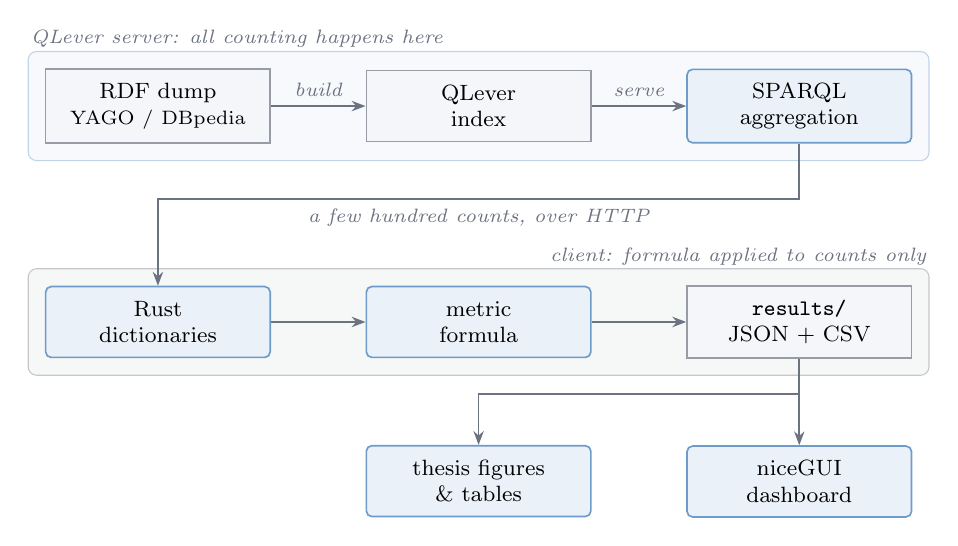
\begin{tikzpicture}[node distance=18mm and 12mm,
    pbox/.style={stage, text width=25mm},
    pstore/.style={store, text width=25mm}]
  % server lane
  \node[pstore]              (kg)     {RDF dump\\\scriptsize YAGO / DBpedia};
  \node[pstore, right=of kg] (index)  {QLever\\index};
  \node[pbox, right=of index](sparql) {SPARQL\\aggregation};
  % client lane
  \node[pbox, below=of kg]       (rust)    {Rust\\dictionaries};
  \node[pbox, right=of rust]     (formula) {metric\\formula};
  \node[pstore, right=of formula](json)    {\texttt{results/}\\JSON + CSV};
  % outputs
  \node[pbox, below=11mm of json]    (dash) {niceGUI\\dashboard};
  \node[pbox, below=11mm of formula] (figs) {thesis figures\\\& tables};

  \draw[flow] (kg) -- node[above, note] {build} (index);
  \draw[flow] (index) -- node[above, note] {serve} (sparql);
  \draw[flow] (sparql.south) -- ++(0,-7mm) -| (rust.north)
        node[pos=.25, below, note] {a few hundred counts, over HTTP};
  \draw[flow] (rust) -- (formula);
  \draw[flow] (formula) -- (json);
  \coordinate (fork) at ($(json.south)+(0,-4.5mm)$);
  \draw[draw=kggrey, line width=.6pt] (json.south) -- (fork);
  \draw[flow] (fork) -- (dash.north);
  \draw[flow] (fork) -| (figs.north);

  \begin{scope}[on background layer]
    \node[fit=(kg)(index)(sparql), draw=kgblue!30, fill=kgblue!4,
          rounded corners=3pt, inner sep=6pt] (server) {};
    \node[fit=(rust)(formula)(json), draw=kggrey!40, fill=kggrey!6,
          rounded corners=3pt, inner sep=6pt] (client) {};
  \end{scope}
  \node[note, anchor=south west, inner sep=1pt] at (server.north west)
       {QLever server: all counting happens here};
  \node[note, anchor=south east, inner sep=1pt] at (client.north east)
       {client: formula applied to counts only};
\end{tikzpicture}}

% ===========================================================================
% Figure: count-of-counts histogram (Chapter 3, efficiency)
% ===========================================================================
\newcommand{\fighistogram}{%
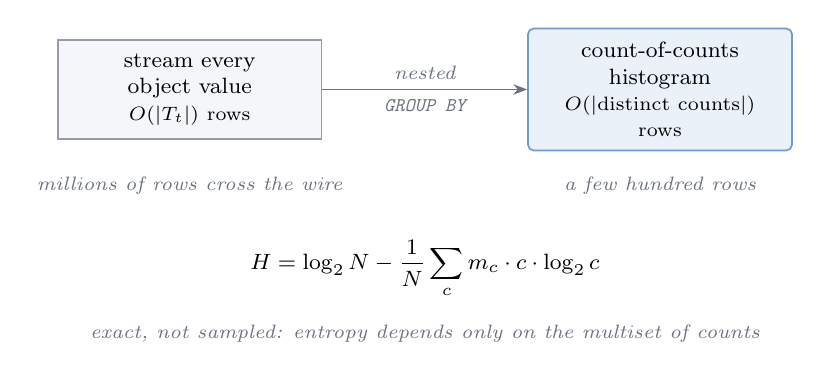
\begin{tikzpicture}
  \node[store, text width=30mm] (naive) {stream every object value\\\scriptsize $O(|T_t|)$ rows};
  \node[stage, right=26mm of naive, text width=30mm] (cc)
       {count-of-counts histogram\\\scriptsize $O(|\text{distinct counts}|)$ rows};
  \draw[flow] (naive) -- node[above, note] {nested} node[below, note] {\texttt{GROUP BY}} (cc);
  % notes share one baseline under the taller box, so they line up
  \coordinate (base) at ($(cc.south)+(0,-2mm)$);
  \node[note, anchor=north] at (naive.south |- base) {millions of rows cross the wire};
  \node[note, anchor=north] at (cc.south |- base) {a few hundred rows};
  \node[font=\footnotesize, anchor=north] (eq) at ($(naive.south |- base)!0.5!(cc.south |- base)+(0,-8mm)$)
       {$H = \log_2 N - \dfrac{1}{N}\displaystyle\sum_{c} m_c \cdot c \cdot \log_2 c$};
  \node[note, below=1mm of eq] {exact, not sampled: entropy depends only on the multiset of counts};
\end{tikzpicture}}

% ===========================================================================
% Figure: subject-window scoping (Chapter 3, metric 10)
% ===========================================================================
\newcommand{\figwindow}{%
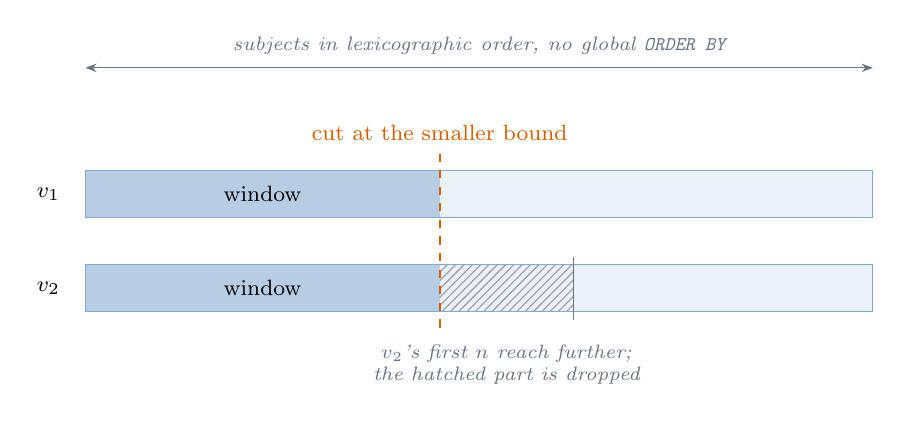
\begin{tikzpicture}[x=1mm, y=1mm, font=\footnotesize]
  % each version lists its subjects in lexicographic order; v1's first n end
  % earlier (x=45) than v2's (x=62), so both are cut at x=45
  \fill[kgpale]    (0,12) rectangle (100,18);
  \fill[kgblue!35] (0,12) rectangle (45,18);
  \draw[kgblue!60] (0,12) rectangle (100,18);
  \fill[kgpale]    (0,0) rectangle (100,6);
  \fill[kgblue!35] (0,0) rectangle (45,6);
  \fill[pattern=north east lines, pattern color=kggrey!70] (45,0) rectangle (62,6);
  \draw[kgblue!60] (0,0) rectangle (100,6);
  \draw[kggrey] (62,-1) -- (62,7);

  \node[anchor=east] at (-2,15) {$v_1$};
  \node[anchor=east] at (-2,3)  {$v_2$};
  \node at (22.5,15) {window};
  \node at (22.5,3)  {window};

  \draw[kgred, line width=.8pt, dashed] (45,-2) -- (45,20);
  \node[kgred, anchor=south] at (45,20.5) {cut at the smaller bound};
  \node[note, anchor=north, text width=46mm] at (53.5,-3)
       {$v_2$'s first $n$ reach further; the hatched part is dropped};

  \draw[{Stealth[length=4pt]}-{Stealth[length=4pt]}, kggrey] (0,31) -- (100,31);
  \node[note, anchor=south] at (50,31.5)
       {subjects in lexicographic order, no global \texttt{ORDER BY}};
\end{tikzpicture}}

% ===========================================================================
% Figure: experiment protocol (Chapter 4)
% Five stages at 20mm text width with 5mm gaps come to ~138mm, inside the
% 146mm text block.
% ===========================================================================
\newcommand{\figprotocol}{%
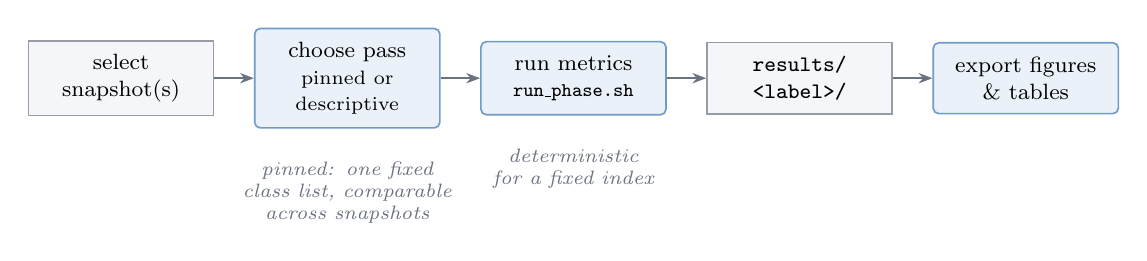
\begin{tikzpicture}[node distance=5mm,
    qbox/.style={stage, text width=20mm},
    qstore/.style={store, text width=20mm}]
  \node[qstore]            (sel)  {select\\snapshot(s)};
  \node[qbox, right=of sel](pass) {choose pass\\\scriptsize pinned or descriptive};
  \node[qbox, right=of pass](run) {run metrics\\\scriptsize\texttt{run\_phase.sh}};
  \node[qstore, right=of run](out){\texttt{results/}\\\texttt{<label>/}};
  \node[qbox, right=of out](read) {export figures\\\& tables};

  \draw[flow] (sel) -- (pass);
  \draw[flow] (pass) -- (run);
  \draw[flow] (run) -- (out);
  \draw[flow] (out) -- (read);

  \node[note, below=3mm of pass, text width=28mm]
       {pinned: one fixed class list, comparable across snapshots};
  \node[note, below=3mm of run, text width=24mm]
       {deterministic for a fixed index};
\end{tikzpicture}}

% ===========================================================================
% Dashboard screenshot slot. Renders the PNG when present, otherwise a marked
% placeholder of the same width, so the document always builds.
% ===========================================================================
\newcommand{\dashshot}[2]{%
  \IfFileExists{figures/#1}{\includegraphics[width=\linewidth]{figures/#1}}{%
    \fbox{\parbox[c][42mm][c]{.97\linewidth}{\centering\footnotesize
      \textcolor{kggrey}{screenshot placeholder}\\[2pt]
      \texttt{figures/#1}\\[4pt] #2}}}%
}


\setlength\footnotemargin{5pt}
% \texttt identifiers cannot hyphenate; give TeX room to reflow the line
% instead of pushing it into the margin.
\setlength{\emergencystretch}{3em}

% Theorem environments
\newtheorem{definition}{Definition}
\newtheorem{example}{Example}

\hyphenation{know-ledge gra-phs SPARQL}

% ---------------------------------------------------------------- metadata
\titleenglish{Efficient Metrics and Visual Analytics for Comparing Evolving Knowledge Graphs}
% \titlegerman{Effiziente Metriken und Visual Analytics zum Vergleich sich entwickelnder Wissensgraphen}
\author{Dharmang~Pambhar}
\supervisor{Prof.~Dr.~Maribel~Acosta}
\assistants{Samuel~García\tlc{}~M.\,Sc.}
\advisor{Samuel~García, M.Sc.}

\courseofstudy{Information Engineering}

\date{21 September 2026}
\location{Heilbronn}

\setcounter{tocdepth}{2}

\addbibresource{bib/IEEEfull.bib}
\addbibresource{bib/literature.bib}

\usepackage{bib}
\usepackage[colorlinks=false,pdfborder={0 0 0}]{hyperref}

\begin{document}%

\pagenumbering{gobble}
\maketitle%
\cleardoublepage

\begin{abstract}
	Knowledge graphs are republished on a schedule, and every release adds, removes
and rewrites facts. Between YAGO~4 and YAGO~4.5.0.2 the class
\texttt{schema:Person} lost 245{,}398 triples and gained 223{,}227 inside a
window of 65{,}182 subjects, while keeping its name and its identifier.
Consumers inherit that change without being told. Plenty of metrics describe one
release; almost nothing describes the difference between two at the scale the
releases actually have.

This thesis builds a catalogue of thirteen metrics spanning the class, entity
and global level, implemented in Rust against any QLever SPARQL endpoint, and a
dashboard that places the results of several releases side by side. Two
components are contributions rather than adoptions. Entropy-weighted PageRank
weights every edge by the normalised property entropy of its predicate, so score
flows through informative relations rather than high-volume bookkeeping ones. An
integer-encoded triple diff with subject-window scoping makes an exact version
comparison possible without a global sort, which SPARQL engines refuse on graphs
of this size.

The evaluation covers seven snapshots: two generations of YAGO, a decade of
DBpedia, and the pre-schema.org YAGO~3 release. The integer encoding runs 2.34 to
6.17 times faster than a string-based baseline and holds its working set in 16 to
19 times less memory, with both paths asserted to return identical results. The
memory figure is what decides feasibility on a 16\,GB client. The metrics show
the two graphs evolving in opposite directions: YAGO replaced 94\% of its class
vocabulary while keeping 72 predicates, whereas DBpedia kept 700 of 740 classes
while 30{,}788 predicates disappeared. Across graphs, DBpedia uses 24 to 92
times more predicates per class than YAGO on all sixteen classes matched
automatically between the latest releases. \texttt{Organization} is the only
class where YAGO~4.5.0.2 and DBpedia 2025 report the same entropy, 14.275 bits
on each side, despite differing in size by a factor of 3.7. Repeating the
comparison against four DBpedia releases and against YAGO~4 shows the agreement
is recent and needed both graphs to change.

\end{abstract}

\acresetall

\tableofcontents
\listoffigures
\listoftables
\startcontent

\chapter{Introduction}
\label{chap:introduction}

\section{Motivation}
\label{sec:motivation}

Knowledge graphs do not hold still. YAGO, DBpedia and Wikidata publish new
releases on a regular schedule, and every release adds facts, removes facts and
rewrites facts that were already there. Between YAGO~4 and YAGO~4.5.0.2 the
class \texttt{schema:Person} lost 245{,}398 triples and gained 223{,}227 inside
a window of 65{,}182 subjects, so roughly three quarters of what the window
described changed while the class kept its name and its identifier. A consumer
of that graph, a question answering system or a search index or a
recommender, inherits the change without being told.

The tooling for describing a single release is mature. Structural quality
metrics, entropy measures over predicate values and importance rankings such as
PageRank all take one graph and return numbers about it. What is missing is a
way to describe the \emph{difference} between two releases at the scale the
releases actually have. YAGO~4 holds 2{,}489{,}858{,}800 triples. Loading two
such graphs into memory to compare them is not an option on ordinary hardware,
and the obvious SPARQL formulation, sorting both graphs and walking them in
parallel, asks the engine for more memory than it has. QLever refused a global
sort on a graph far smaller than YAGO when we tried it.

So the practical question is narrower than it first appears. Not \emph{can we
compare two knowledge graphs}, which is easy on toy data, but \emph{can we
compute a useful, exact comparison of two billion-triple graphs through a SPARQL
endpoint, on a laptop}. That question drives this thesis. It also explains why
efficiency appears in the title next to metrics: a metric nobody can afford to
run is not a metric.

A second gap sits beside the first. Numbers alone do not show evolution. Five
snapshots across two knowledge graphs produce more values than anyone reads in a
table, and the interesting behaviour lives in how a value moves across releases
rather than in any single value. The comparison therefore needs a visual front
end, and the front end needs to be honest about what it is showing. A blank cell
in a comparison must mean something definite, and this thesis takes some care
over that point, because during development it turned out that the same blank
cell could mean three different things.

\section{Research Objectives}
\label{sec:research_objectives}

The thesis answers four questions.

\begin{description}
  \item[RQ1] Which metrics characterise a knowledge graph snapshot at the class,
    entity and global level, and can they be computed exactly over a
    billion-triple graph through a SPARQL endpoint rather than over a local
    dump?
  \item[RQ2] How do those metrics change between two versions of the same
    knowledge graph, and where in the graph does the change concentrate?
  \item[RQ3] Can a version comparison be made cheap enough to run on commodity
    hardware, and by how much does an integer encoding of triples improve on the
    obvious string-based implementation?
  \item[RQ4] What do the same metrics report when applied across two different
    knowledge graphs rather than two versions of one, and what breaks when they
    are?
\end{description}

RQ1 and RQ2 are the descriptive core. RQ3 is the efficiency claim, and it is the
one question here with a hard number attached. RQ4 is deliberately last, because
the cross-graph case is where the assumptions behind the other three stop
holding, and saying exactly how they stop holding is part of the contribution.

\section{Contributions}
\label{sec:contributions}

This thesis contributes the following.

\begin{itemize}
  \item \textbf{A catalogue of thirteen metrics over three analysis levels},
    implemented in roughly 2{,}350 lines of Rust across 19 modules, each
    expressed as SPARQL aggregation plus a formula applied to the counts. Every
    metric runs against any QLever endpoint and writes JSON and CSV, so results
    are reproducible and machine readable.
  \item \textbf{Entropy-weighted PageRank}, a variant in which each edge carries
    a weight equal to the normalised property entropy of its predicate, so
    importance flows through informative relations rather than through
    high-volume bookkeeping predicates. On YAGO~4 the weighting converges in 43
    iterations where the unweighted baseline fails to converge in 100, and it
    moves 5{,}327 of 5{,}372 sampled nodes.
  \item \textbf{An integer-encoded triple diff with subject-window scoping},
    which makes an exact version comparison tractable without a global sort. The
    encoding runs up to 6.2 times faster than a string-based baseline and holds
    the working set in up to 19 times less memory, with both paths asserted to
    produce identical results.
  \item \textbf{A visual analytics dashboard} covering all thirteen metrics
    across seven snapshots, including a treatment of missing data that
    distinguishes a measured zero from an unmeasured class.
  \item \textbf{An evaluation over seven snapshots} spanning a decade of DBpedia
    and three generations of YAGO, plus a cross-graph comparison of two YAGO
    releases against four DBpedia releases on up to twenty-three automatically
    matched classes.
\end{itemize}

Two components are adopted rather than claimed. Entropy-weighted type importance
(ETImp) and classic PageRank both come from the Knowgly work and serve here as
baselines. Chapter~\ref{chap:approach} marks them as such where they appear.

\section{Organization}
\label{sec:organization}

Chapter~\ref{chap:relatedwork} reviews quality metrics, ranking, knowledge graph
evolution and prior work on version and cross-graph comparison, and ends by
naming the gaps this thesis fills. Chapter~\ref{chap:approach} fixes the
notation, describes the pipeline and defines all thirteen metrics, then presents
entropy-weighted PageRank and the three techniques that make the computation
affordable. Chapter~\ref{chap:experiments} describes the five snapshots, the
three machines and the measurement protocol, then reports five experiments with
their results and what they mean. Chapter~\ref{chap:conclusion} answers the four
research questions, states the limitations honestly and lists the work that
follows from here.

\chapter{Related Work}
\label{chap:relatedwork}

This chapter covers four bodies of work. Section~\ref{sec:rw_kgs} introduces the
knowledge graphs this thesis measures. Section~\ref{sec:rw_quality_metrics}
reviews metrics that describe one snapshot, and
Section~\ref{sec:rw_ranking} the ranking measures that
Chapter~\ref{chap:approach} builds on. Section~\ref{sec:rw_evolution} covers work
on how knowledge graphs change, and Section~\ref{sec:rw_comparison} the
comparison of versions and of different graphs.
Section~\ref{sec:rw_gaps} states what none of it provides.

\section{Knowledge Graphs and Their Releases}
\label{sec:rw_kgs}

A knowledge graph stores facts as RDF triples~\cite{cyganiak2014rdf} and exposes
them to queries through SPARQL~\cite{harris2013sparql}. Hogan et
al.~\cite{hogan2021knowledge} survey the field and the design decisions that
separate one graph from another.

The two graphs measured here have long release histories. YAGO began by combining
Wikipedia categories with WordNet~\cite{suchanek2007yago,miller1995wordnet}, gained spatial and
temporal facts in YAGO2~\cite{hoffart2013yago2}, and became multilingual in
YAGO3~\cite{mahdisoltani2015yago3}. YAGO~4 broke with all of
that~\cite{tanon2020yago}: it dropped the WordNet and Wikipedia-category
taxonomy and adopted schema.org~\cite{guha2016schema} classes with Wikidata
identifiers. YAGO~4.5~\cite{suchanek2024yago45} keeps the schema.org top level
and adds a large part of the Wikidata taxonomy beneath it, subject to logical
constraints that keep classes and instances apart, which is why its class count
grows from about ten thousand to over a hundred thousand. That break
matters to this thesis in a concrete way, because it means YAGO~3 and YAGO~4
share almost no class names, and Chapter~\ref{chap:experiments} reports what
happens when a per-class metric meets that discontinuity.

DBpedia extracts structured data from Wikipedia
infoboxes~\cite{auer2007dbpedia,bizer2009dbpedia}, and the release used
here is described by Lehmann et al.~\cite{lehmann2015dbpedia}. Since 2020
DBpedia has been published through a redesigned, largely automated release
cycle with monthly snapshots~\cite{hofer2020dbpedia}, which is the source of the
2022 and 2025 releases measured here. Wikidata is the
third large open graph~\cite{vrandecic2014wikidata,erxleben2014introducing};
this thesis does not measure it, and Section~\ref{sec:future_work} says why that
is the obvious next step.

All queries here run through QLever~\cite{bast2017qlever}, a SPARQL engine that
answers from a precomputed index and can hold a billion-triple graph on a single
machine. That capability is what makes the endpoint-based approach of
Chapter~\ref{chap:approach} possible at all.

\section{Quality and Importance Metrics}
\label{sec:rw_quality_metrics}

Zaveri et al.~\cite{zaveri2016quality} survey linked data quality assessment and
organise it into dimensions such as completeness, consistency and conciseness.
Färber et al.~\cite{farber2018linked} apply a comparable framework to DBpedia,
Freebase, OpenCyc, Wikidata and YAGO side by side, which is the closest prior
work to the cross-graph comparison in Section~\ref{sec:exp5}. Their comparison is
a one-off study of a fixed set of releases rather than a repeatable measurement,
and it does not track a graph across its own versions.

Seo et al.~\cite{seo2024structural} propose structural quality metrics computed
from the graph topology. Their measures describe one snapshot and say nothing
about a successor.

Dataset profiling tools share that limitation. LODStats~\cite{auer2012lodstats}
computes statistics such as class and property usage over a stream of RDF
statements, and Duan et al.~\cite{duan2011apples} define structuredness, a
measure of how uniformly the instances of a class use the properties of that
class, to show that benchmark data looks nothing like real RDF data. Both are
close in spirit to the class-level metrics of this thesis, and structuredness in
particular asks a question related to class entropy. Both describe one dataset
at a time.

The direct ancestor of this work is Knowgly, by García and
Bobed~\cite{garcia2025information}. Knowgly measures how much information a
predicate carries for a class, using property entropy and entropy-weighted type
importance, and it establishes the pattern this thesis reuses: SPARQL performs
the counting, the host language holds the aggregated counts and applies the
formula. Chapter~\ref{chap:approach} adopts that pattern and two of its metrics
as baselines. What Knowgly does not do is compare two graphs. Every Knowgly
number describes one endpoint, and nothing in it addresses what changes between
releases.

Shannon's definition of entropy~\cite{shannon1948mathematical} underlies metrics
2, 3, 4 and 7. Section~\ref{subsec:count_of_counts} shows how to compute it exactly
over a billion-triple graph without streaming the values.

\section{Entity and Predicate Ranking}
\label{sec:rw_ranking}

PageRank~\cite{page1999pagerank} ranks nodes by the stationary distribution of a
random walk. Applied to RDF without modification it treats every edge alike, so
a predicate that appears on every entity contributes as much as one that appears
rarely. On YAGO~4 this is a real problem: \texttt{schema:gender} carries a
normalised property entropy of 0.034, while \texttt{schema:geo} carries 1.000,
and unweighted PageRank cannot tell them apart.

Menendez et al.~\cite{menendez2018ranking} decouple ranking from raw
degree and rank entities by the information they carry, which motivates metric~5
in this thesis. Section~\ref{sec:entropy_weighted_pagerank} takes the next step
and pushes the information measure into the edge weights of the walk itself.

Weighting PageRank is not new in itself. Xing and Ghorbani~\cite{xing2004weighted}
distribute rank in proportion to the in-link and out-link popularity of the
target pages, and Langville and Meyer~\cite{langville2004deeper} survey the
variants and the conditions under which the power iteration converges. What
differs here is the source of the weight: it comes from the predicate that
labels the edge, measured by its entropy over the whole graph, rather than from
the link structure around the node.

\section{Knowledge Graph Evolution}
\label{sec:rw_evolution}

Polleres et al.~\cite{polleres2023knowledge} describe how knowledge evolves in
open knowledge graphs and argue that consumers need to understand change rather
than only consume the latest release. The ISWS report on evolution and
preservation~\cite{isws2019evolution} makes a similar case from the archival
side.

Käfer et al.~\cite{kafer2013observing} measured linked data dynamics empirically
by monitoring documents over time and reporting how often they change. Their unit
of observation is the document, not the class or the predicate, so the results
say how much a dataset churns without saying which part of the schema moved.

Ontology change has its own literature. Flouris et
al.~\cite{flouris2008ontology} classify the kinds of change an ontology can
undergo, and Noy and Musen~\cite{noy2004ontology} address versioning inside an
ontology management framework. Both work at the schema level and assume the
schema is small enough to reason about directly, which is true of a hand-built
ontology and false of DBpedia's 54{,}933 predicates.

\section{Comparing Versions and Comparing Graphs}
\label{sec:rw_comparison}

Papavasileiou et al.~\cite{papavasileiou2013high} detect high-level changes in
RDF(S) knowledge bases, lifting low-level triple additions and deletions into
meaningful operations. Roussakis et al.~\cite{roussakis2015flexible} generalise
this into a framework for defining and detecting changes over evolving RDF
datasets. Zeginis et al.~\cite{zeginis2011deltas} study how to compute the
delta between two RDF/S knowledge bases and how inferred triples change its
size. All three operate over datasets held locally, and all assume the two
versions can be loaded and traversed together.

The closest relative of metric~10 is the DBpedia Wayback
Machine~\cite{fernandez2015dbpedia}, which reconstructs historical DBpedia states
and diffs them using integer-encoded triples. Replacing IRIs and literals by
integer identifiers through a dictionary is standard practice in RDF storage,
from the RDF-3X engine~\cite{neumann2010rdf3x} to the HDT exchange
format~\cite{fernandez2013hdt}. This thesis takes the same encoding
idea and pairs it with a scoping scheme that removes the need for a global sort,
which is what allows the diff to run against a live endpoint rather than a
prepared archive.

The closest relative of metric~13 is Ringler and
Paulheim~\cite{ringler2017one}, who ask whether DBpedia, YAGO and Wikidata are
interchangeable and conclude that they are not. Their comparison is manual and
fixed in time. This thesis automates the class matching and reports the same
comparison as a repeatable metric, at the cost of matching classes by local name
rather than by instance-level alignment. Section~\ref{sec:exp5} is explicit about
what that costs.

\section{Summary of Gaps}
\label{sec:rw_gaps}

Three gaps follow from the above, and this thesis addresses each.

\textbf{Per-snapshot metrics are not tracked across versions.} Knowgly, Seo et
al.\ and the quality surveys all describe a single graph. A value becomes far
more informative when read next to the same value from the previous release, and
no existing tool computes a metric catalogue across a release series.

\textbf{Diffing work assumes local dumps.} Papavasileiou et al., Roussakis et
al., Zeginis et al.\ and the DBpedia Wayback Machine all operate on data the tool
controls. None
of them answers what an analyst can compute when the graph is only reachable
through a SPARQL endpoint, which is the normal situation for a billion-triple
graph on ordinary hardware.

\textbf{No combined metric and visual analytics pipeline exists.} Visual
analytics couples automatic analysis with interactive
visualisation~\cite{keim2008visual}, and it has reached large knowledge graphs:
the SHACL Dashboard of Mäkelburg et al.~\cite{makelburg2025shacl} makes
validation reports over large graphs explorable where reading them by hand is
infeasible. It analyses the quality of one graph against its shapes, not the
difference between releases. Comparison results are otherwise reported as
tables in papers. Nothing takes a metric catalogue across
several versions of several graphs and presents it so the movement is visible.
Chapter~\ref{chap:experiments} shows that the presentation is not cosmetic: the
same blank cell in a comparison can mean a measured zero, an unmeasured class or
a class that does not exist in that release, and a reader who cannot tell them
apart will draw the wrong conclusion.

\chapter{Approach}
\label{chap:approach}

This chapter describes what is computed and how. Section~\ref{sec:preliminaries}
fixes the notation, Section~\ref{sec:architecture} explains the shape of the
pipeline, and Sections~\ref{sec:class_level_metrics}--\ref{sec:global_metrics}
define the thirteen metrics grouped by the level of the graph they describe.
Section~\ref{sec:entropy_weighted_pagerank} presents the entropy-weighted
PageRank variant proposed by this thesis, and
Section~\ref{sec:efficient_computation} covers the techniques that make the
computation tractable on billion-triple graphs.

\section{Preliminaries}
\label{sec:preliminaries}

A knowledge graph is a set of RDF triples $T \subseteq (I \cup B) \times I
\times (I \cup B \cup L)$, where $I$ are \acp{IRI}, $B$ blank nodes and $L$
literals. A triple $(s, p, o)$ states that subject $s$ stands in relation $p$ to
object $o$. Throughout this thesis the following symbols are used:

\begin{itemize}
  \item $T$ --- the set of triples of one snapshot, $|T|$ its cardinality;
  \item $S$ --- the set of distinct subjects, $O$ the set of distinct objects;
  \item $P$ --- the set of distinct predicates;
  \item $C$ --- the set of classes, that is the objects of \texttt{rdf:type} triples;
  \item $E$ --- the set of typed entities, $E_t \subseteq E$ those of class $t$.
\end{itemize}

An entity may carry several types, so the sets $E_t$ overlap and
$\sum_{t \in C} |E_t| \geq |E|$ in general. This matters when reading
Section~\ref{sec:class_level_metrics}: class shares are fractions of $|E|$ but
need not sum to one.

Two versions of the same knowledge graph are written $v_1$ and $v_2$ with triple
sets $T_1$ and $T_2$; two different knowledge graphs are written $A$ and $B$.
The distinction is not cosmetic. Two versions of one graph share their \ac{IRI}
namespace, so their triples can be compared directly; two different graphs
generally do not, and Section~\ref{sec:global_metrics} treats them with separate
metrics for exactly that reason.

All metrics are computed over data served by QLever~\cite{bast2017qlever}, a
SPARQL engine that answers queries from a precomputed index. Every metric in
this chapter is therefore expressible as one or more SPARQL queries plus a
formula applied to their results.

\section{Architecture}
\label{sec:architecture}

The pipeline follows the pattern established by Knowgly~\cite{garcia2025information}:
\emph{SPARQL performs the counting, the host language holds the aggregated counts
in dictionaries and applies the formula, and a separate layer visualises the
result}. Concretely it has four stages:

\begin{enumerate}
  \item a QLever index of one snapshot of a knowledge graph, served as a SPARQL
        endpoint over HTTP;
  \item a set of counting queries, one or a few per metric, evaluated on the
        server so that no triple ever crosses the network unnecessarily;
  \item a Rust~\cite{matsakis2014rust} program that collects the counts into hash maps, applies the
        metric formula, and writes the result as JSON and CSV;
  \item a niceGUI dashboard that reads those files and renders them.
\end{enumerate}

Figure~\ref{fig:pipeline} shows the four stages and where the data volume drops.

\begin{figure}[htbp]
  \centering
  \figpipeline
  \caption[\entrydesc{The measurement pipeline}{Counting on the server, formulas in Rust, results to JSON and the dashboard}]{The measurement pipeline. Hundreds of
    millions of triples are aggregated inside the engine; only a few hundred
    counts cross the network to the client, which applies the formula and writes
    the result. The dashboard and the figures in
    Chapter~\ref{chap:experiments} both read the same files.}
  \label{fig:pipeline}
\end{figure}

Splitting the work this way is what keeps the approach applicable to graphs of
this size. The expensive part of every metric is an aggregation over hundreds of
millions of triples, which the engine can answer from its index; what remains is
arithmetic over a few hundred or a few thousand numbers, which is trivial in any
language. The role of Rust is therefore not raw speed in the formula itself but
predictable memory behaviour in the two places where data volume does reach the
client: the triple diff of Section~\ref{subsec:integer_encoding} and the
PageRank iteration of Section~\ref{sec:entropy_weighted_pagerank}.

The endpoint is not compiled in. It is read from the environment, so the same
binary runs against a laptop, a server on the local network, or a university
virtual machine without modification. A second endpoint may be supplied for the
metrics that compare two graphs. Each run may additionally be given a label
naming the snapshot being measured; results are then written to a directory of
that name, which is the mechanism the trajectory metric of
Section~\ref{sec:global_metrics} uses to find several versions of the same
measurement.

\section{Class-Level Metrics}
\label{sec:class_level_metrics}

Class-level metrics describe what kinds of things a graph contains and which
predicates characterise each kind.

\subsection{Class Population and Share}

The most basic question about a snapshot is what is in it. For a class $t$,

\begin{equation}
  \mathrm{share}(t) = \frac{|E_t|}{|E|}
  \label{eq:share}
\end{equation}

gives the fraction of all typed entities belonging to $t$. Both quantities come
from a single grouped count. Tracked across versions, the share exposes which
classes grow, shrink or vanish, and it normalises for overall growth: a class
can double in absolute size while losing share, which is a different fact about
the graph than simply getting bigger.

\subsection{Property Entropy per Type}

Population says nothing about how well a class is described. For that we ask, for
one class $t$ and one predicate $p$, how varied the values of $p$ are. Let $P(o)$
be the relative frequency of value $o$ among all values $p$ takes on entities of
$t$. The Shannon entropy~\cite{shannon1948mathematical} of that distribution is

\begin{equation}
  \mathrm{EntF}(p, t) = - \sum_{o} P(o) \log_2 P(o).
  \label{eq:entf}
\end{equation}

A predicate whose values are spread over many distinct objects --- a birth date,
where nearly every person differs --- scores high and carries real information. A
predicate dominated by one value --- a gender field with two outcomes, or a
constant marker --- scores near zero. Entropy is measured in bits and is bounded
above by $\log_2 D$, where $D$ is the number of distinct values, with equality
when all values are equally frequent.

Computing Equation~\ref{eq:entf} naively means retrieving every object value of
every predicate of every class, which is prohibitive at this scale.
Section~\ref{subsec:count_of_counts} shows how to obtain it exactly from a
result of a few hundred rows.

\subsection{Entropy-Weighted Type Importance}

Property entropy measures how informative a predicate's values are, but not
whether the predicate is characteristic of the class. The complementary signal is
the \ac{ETImp} measure of Knowgly~\cite{garcia2025information}, a TF--IDF
analogue for predicates:

\begin{equation}
  \mathrm{ETImp}(p, t) = \mathrm{EF}_p(p, t) \cdot
    \log_2 \frac{|E_t|}{\mathrm{EF}_p(p, t)},
  \label{eq:etimp}
\end{equation}

where $\mathrm{EF}_p(p,t)$ is the number of distinct entities of class $t$ that
use $p$. A predicate used by every entity of the class contributes
$\log_2 1 = 0$: universal predicates are uninformative precisely because they do
not discriminate.

Neither signal suffices alone. A predicate every entity carries scores zero on
\ac{ETImp} regardless of how diverse its values are; a predicate with a single
repeated value scores near zero on \ac{EntF} regardless of how characteristic it
is. This thesis therefore combines them as a weighted geometric mean:

\begin{equation}
  \mathrm{EntETImp}(p, t) = \mathrm{EntF}(p, t)^{w} \cdot
                            \mathrm{ETImp}(p, t)^{1 - w},
  \qquad w = 0.75.
  \label{eq:entetimp}
\end{equation}

The geometric mean is chosen deliberately over an arithmetic one: it collapses to
zero whenever either factor is zero, which is the desired semantics here. A
predicate must be both typical of the class and informative in its values to rank
highly. The weight $w$ favours the entropy term; it is a parameter, and every
result in Chapter~\ref{chap:experiments} uses $w = 0.75$.

\subsection{Class Entropy}

The two preceding metrics are defined per predicate. Aggregating to the class
gives one number describing how diverse a class is as a whole:

\begin{equation}
  H(t) = - \sum_{o} P(o) \log_2 P(o),
  \label{eq:class_entropy}
\end{equation}

where $P(o)$ now ranges over \emph{all} object values occurring on entities of
$t$, irrespective of predicate. A class whose entities all look alike scores low;
a class of varied, richly described entities scores high.

The same quantity is also computed over the predicates used by the class rather
than the object values. The two are reported together because they can diverge in
an informative way: a class may take highly varied values through a very narrow
set of predicates, which says something quite different about the modelling than
a class described by many predicates with repetitive values.

\section{Entity-Level Metrics}
\label{sec:entity_level_metrics}

Entity-level metrics move from kinds of things to individual things.

\subsection{Entity Informativeness}

Following the intuition behind InfoRank~\cite{menendez2018ranking} --- that
important entities have a lot recorded about them --- the informativeness of an
entity $v$ is the normalised count of its datatype properties:

\begin{equation}
  \mathrm{IR}(v) = \frac{\mathrm{dtp}(v)}{\sum_{u} \mathrm{dtp}(u)},
  \label{eq:inforank}
\end{equation}

where $\mathrm{dtp}(v)$ is the number of triples of $v$ whose object is a
literal. Literals are what is counted, and the restriction is deliberate: a link
to another entity records who $v$ is related to, whereas a literal records
something \emph{about} $v$. The measure needs a single grouped aggregation and no
iteration, which makes it one of the cheapest metrics in the catalogue. Across
versions it distinguishes entities that are being actively enriched from those
that have been abandoned.

\subsection{Object Diversity}

Entropy weights values by how often they occur. The complementary measure counts
them without weighting:

\begin{equation}
  \mathrm{OD}(p, t) = |\{\, o : (e, p, o) \in T \text{ and } e \in E_t \,\}|,
  \label{eq:objdiv}
\end{equation}

the number of distinct objects a predicate takes within a class. Reported
alongside the total number of such triples, the ratio
$\mathrm{OD}(p,t) / |\{(e,p,o) \in T : e \in E_t\}|$ states whether values are
mostly unique (ratio near one) or heavily reused (ratio near zero). This is an
exact count rather than an information-theoretic quantity, and it serves as a
sanity check on the entropy metrics: the two should agree on the extremes and may
legitimately disagree in between.

\section{Global Metrics}
\label{sec:global_metrics}

Global metrics describe the graph as a whole and, in most cases, the difference
between two graphs.

\subsection{Graph Size and Shape}
\label{subsec:shape_metric}

The foundation table of every snapshot: the counts $|T|$, $|S|$, $|O|$, $|P|$,
$|C|$ and $|E|$, together with

\begin{equation}
  \mathrm{density} = \frac{|T|}{|E|},
  \qquad
  \overline{\deg}^{\,+} = \frac{|T|}{|S|},
  \qquad
  \overline{\deg}^{\,-} = \frac{|T|}{|O|}.
  \label{eq:shape}
\end{equation}

Density is triples per entity; the two degree averages are the mean out- and
in-degree. None of these is surprising in isolation. Their value is comparative:
computed for every version and every graph, their deltas form the growth table
against which all other comparisons are read. A rise in absolute triple count
means one thing if density rose with it and quite another if density fell.

\subsection{Triple-Level Diff}

The core of any comparison between two versions is the set difference between
their triples:

\begin{equation}
  \mathrm{Added} = T_2 \setminus T_1,
  \qquad
  \mathrm{Deleted} = T_1 \setminus T_2,
  \qquad
  \mathrm{Unchanged} = T_1 \cap T_2.
  \label{eq:diff}
\end{equation}

Conceptually this is elementary. Making it computable over graphs of a billion
triples, through a SPARQL endpoint rather than over local dumps, is not; that is
the subject of Sections~\ref{subsec:integer_encoding}
and~\ref{subsec:subject_window}. This metric applies only to two versions of the
same graph. Two different knowledge graphs generally use disjoint \ac{IRI}
namespaces, and Equation~\ref{eq:diff} evaluated across them reports every triple
of one side as added --- arithmetically correct and entirely without meaning.

\subsection{Class-Level Change Rate}
\label{subsec:churn_metric}

The diff says how much changed; it does not say where. For each class $t$, let
$A_t$ and $D_t$ be the added and deleted triples whose subject belongs to $t$,
and $T_t(v_1)$ its triples in the older version. The churn of the class is

\begin{equation}
  \mathrm{churn}(t) = \frac{|A_t| + |D_t|}{|T_t(v_1)|}.
  \label{eq:churn}
\end{equation}

This distinguishes two situations a global diff conflates: a graph in which
everything drifted slightly, and a graph in which a few classes were rewritten
while the rest stood still. Because it reuses the diff machinery with the scope
restricted to one class, it costs little beyond the diff itself.

\subsection{Vocabulary and Schema Evolution}

At the schema level the same set difference applies to the class and predicate
vocabularies:

\begin{equation}
  C_{\mathrm{added}} = C_2 \setminus C_1,
  \qquad
  C_{\mathrm{removed}} = C_1 \setminus C_2,
  \label{eq:vocab}
\end{equation}

and analogously for $P$. Presence in the vocabulary is, however, a weak signal on
its own: a term can be introduced and remain almost unused for a version or two.
Each newly added predicate is therefore reported together with the number of
triples that actually use it in $v_2$, which measures adoption rather than mere
declaration.

\subsection{Metric Trajectories}

The framework layer, and the reason every metric writes its result to a labelled
directory. For a metric $m$ and consecutive versions $v_i$,

\begin{equation}
  \Delta m(v_i) = m(v_{i+1}) - m(v_i).
  \label{eq:trajectory}
\end{equation}

The implementation is deliberately generic over $m$: it reads the stored results
of a metric for a list of labelled snapshots, flattens each to its numeric
leaves, and reports the series and its deltas for every value present in all
snapshots. Values that appear in only some snapshots are counted and reported
separately, since their appearance or disappearance is itself a finding. A metric
added later requires no change to this component.

\subsection{Cross-KG Class Comparison}

Finally, the same class may exist in two different knowledge graphs, and its
metric values can be placed side by side:

\begin{equation}
  \Delta m(t) = m_A(t) - m_B(t).
  \label{eq:crosskg}
\end{equation}

Classes are matched at the schema level, by local name. This is a real
limitation and is stated as such: aligning the \emph{instances} of two knowledge
graphs through \texttt{owl:sameAs} links is impractical at this scale, so no
union, overlap or merge gain is estimated here, unlike the analysis of Ringler
and Paulheim~\cite{ringler2017one}. What the comparison does show is how
differently two graphs model and populate the same concept: how many entities
they assign to it, how many predicates they use to describe it, and how diverse
the resulting values are.

\section{Entropy-Weighted PageRank}
\label{sec:entropy_weighted_pagerank}

Classic PageRank~\cite{page1999pagerank} treats every link alike: a node
distributes its rank uniformly over its outgoing edges. In a knowledge graph that
assumption is questionable, because the edges are typed and the types differ
enormously in what they tell us. An edge labelled with a near-constant predicate
connects two nodes without saying much about either; an edge labelled with a
highly varied predicate is far more specific. Knowgly~\cite{garcia2025information}
makes a related observation and weights its links using an InfoRank-derived
factor, and weighted PageRank in general goes back at least to Xing and
Ghorbani~\cite{xing2004weighted}, who weight links by the popularity of the
pages they join.

This thesis proposes a simpler variant: weight each edge by the property entropy
of its predicate, the quantity already defined in Equation~\ref{eq:entf}. Let

\begin{equation}
  w(p) = \frac{\mathrm{EntF}(p)}{\max_{q \in P} \mathrm{EntF}(q)}
  \label{eq:weight}
\end{equation}

be the entropy of predicate $p$ over the whole graph, normalised into $[0, 1]$ by
the largest entropy of any predicate. The rank update becomes

\begin{equation}
  \mathrm{PR}(v) = (1 - d) + d \sum_{u \rightarrow v}
                   w(p_{uv}) \cdot \frac{\mathrm{PR}(u)}{\mathrm{outdeg}(u)},
  \label{eq:entropy_pagerank}
\end{equation}

with damping factor $d = 0.85$. Rank now flows preferentially through
informative predicates. Setting $w(p) = 1$ for all $p$ recovers classic PageRank
exactly, which is convenient: the baseline is not a separate implementation but
the same code path with uniform weights, so the two rankings are computed over an
identical edge set and are directly comparable.

Three properties of Equation~\ref{eq:entropy_pagerank} deserve comment. First,
the weight is a property of the predicate and is computed over the entire graph,
not over whatever subgraph the ranking is run on; it is a statement about what
the predicate means in this knowledge graph, not about the sample. Second, only
edges between entities participate --- triples with literal objects are not
links, and including them would let rank leak into values. Third, the
normalisation divides by $\mathrm{outdeg}(u)$, the number of outgoing edges,
rather than by the sum of outgoing weights. This means a node whose outgoing
edges are all low-entropy passes on less total rank than it received, so the
weighted variant is not rank-preserving in the way classic PageRank is. This is a
deliberate consequence: a node that connects to the rest of the graph only
through uninformative predicates should not confer as much importance. It is also
a clear point of comparison against a weight-normalised alternative, and
Chapter~\ref{chap:experiments} reports the difference between the two rankings
rather than either in isolation.

\section{Efficient Computation}
\label{sec:efficient_computation}

The definitions above are straightforward. Evaluating them over graphs of one to
two billion triples, through a query endpoint, on commodity hardware, is where
the work lies. Three techniques carry most of the weight.

\subsection{Entropy from Count-of-Counts Histograms}
\label{subsec:count_of_counts}

A direct evaluation of Equation~\ref{eq:entf} requires the frequency of every
distinct object value of a predicate within a class. For a predicate such as a
label on a class with millions of members, that is millions of rows transferred
and counted --- per predicate, per class.

The observation that removes this cost is that entropy depends only on the
\emph{multiset} of counts, never on the values that carry them. Two predicates
whose value distributions are permutations of one another have identical entropy.
It is therefore sufficient to know, for each multiplicity $c$, how many distinct
values occur exactly $c$ times. Statisticians call this the frequency of
frequencies, and it is the same summary Good~\cite{good1953population} used to
estimate the population of unseen species. Writing $m_c$ for that number, and
$N = \sum_c m_c \, c$ for the total number of value occurrences, the entropy of
Equation~\ref{eq:entf} can be rewritten as

\begin{equation}
  H = \log_2 N - \frac{1}{N} \sum_{c} m_c \cdot c \cdot \log_2 c.
  \label{eq:entropy_histogram}
\end{equation}

\begin{proof}[Derivation]
With $P(o) = c_o / N$ for a value occurring $c_o$ times,
\[
  H = -\sum_{o} \frac{c_o}{N} \log_2 \frac{c_o}{N}
    = \log_2 N - \frac{1}{N} \sum_{o} c_o \log_2 c_o ,
\]
and grouping the values by their multiplicity $c$ replaces the sum over values
by a sum over multiplicities weighted by $m_c$.
\end{proof}

Figure~\ref{fig:histogram} contrasts the two formulations.

\begin{figure}[htbp]
  \centering
  \fighistogram
  \caption[\entrydesc{Count-of-counts histogram}{Exact entropy from a few hundred rows instead of millions of values}]{Computing entropy from a count-of-counts
    histogram. Streaming every object value transfers millions of rows per
    predicate and class; a nested \texttt{GROUP BY} returns one row per distinct
    multiplicity, typically a few hundred. The result is exact, not sampled,
    because entropy depends only on the multiset of counts.}
  \label{fig:histogram}
\end{figure}

The histogram $(c, m_c)$ is obtained from a nested grouped query: the inner query
counts occurrences per value, the outer counts values per occurrence count. Both
aggregations run on the server, and the result has as many rows as there are
distinct multiplicities --- typically a few hundred, sometimes fewer than ten.
The number of distinct values, needed for Equation~\ref{eq:objdiv}, falls out of
the same histogram as $\sum_c m_c$.

The essential point is that this is not an approximation. Equation~\ref{eq:entropy_histogram}
is an algebraic identity, so the entropy obtained from the histogram is exactly
the entropy of the full distribution. The saving is in transport and client-side
work, not in fidelity, which distinguishes it from sampling-based estimators.

\subsection{Integer-Encoded Triple Sets}
\label{subsec:integer_encoding}

The set operations of Equation~\ref{eq:diff} are the one place where triples
themselves, rather than counts, must reach the client. Comparing them as strings
is expensive in both time and space: each triple carries three \acp{IRI} of
typically 30 to 60 bytes, and every set operation hashes all three.

Instead, each distinct term encountered on either side is interned once into a
32-bit integer, with a single dictionary shared across both versions so that
equal strings receive equal identifiers. A triple becomes a triple of integers
occupying twelve bytes, and the comparison reduces to sorting two integer arrays
and merging them linearly. String data is touched exactly once, during
interning; the set operations themselves never look at a byte of text.

Both this path and a naive implementation using hash sets of string triples are
implemented, and Chapter~\ref{chap:experiments} benchmarks them against each
other. The two are also cross-checked at run time: the implementation asserts
that both produce identical added, deleted and unchanged counts, so the reported
speedup cannot silently be a speedup of the wrong answer.

\subsection{Subject-Window Scoping}
\label{subsec:subject_window}

Even encoded, the full triple set of a billion-triple version does not fit in the
memory of the machines used here, so the diff must run over a well-defined
subset. The subset has to satisfy two conditions: it must be cheap to obtain, and
both versions must return \emph{the same} subset, or the difference between them
is an artefact of the sampling rather than of the data.

A bare \texttt{LIMIT} fails the second condition, since the engine may return any
rows it likes. The obvious repair, ordering the triples and taking a prefix,
fails the first: ordering by subject, predicate and object forces the server to
sort the entire graph before it can return the first row. Measured on a graph of
roughly 1.5 billion triples, QLever attempted to allocate 12.7\,GB for such a
query and aborted.

Figure~\ref{fig:window} shows the scheme adopted instead, a
\emph{subject window}.

\begin{figure}[htbp]
  \centering
  \figwindow
  \caption[\entrydesc{Subject-window scoping}{How metric 10 compares two versions without a global sort}]{Subject-window scoping for metric~10. Each
    version returns its lexicographically first $n$ subjects, which is far
    cheaper than ordering every triple. Both prefixes are then cut at the
    smaller bound, so the two versions cover exactly the same subjects and the
    difference between them is the data rather than the sampling.}
  \label{fig:window}
\end{figure}

Ordering a list of
distinct subjects is far cheaper than ordering every triple, so from each version
the lexicographically first $n$ subjects are retrieved. The two prefixes are then
truncated at whichever ends earlier, and their union forms the window. Every
triple of every subject in the window is fetched by naming the subjects
explicitly, which requires no ordering at all, since naming them already
determines the result set exactly.

The window has a property worth stating precisely: within it, both versions are
covered \emph{completely}. Any triple of any subject in the window is present in
the fetched data for whichever versions contain it, so the diff restricted to the
window is exact --- including for entities that appear in one version and not the
other. Truncating at the earlier of the two upper bounds is what guarantees this;
beyond that bound one version would be missing subjects the other has, and their
absence would be indistinguishable from deletion. The diff is thus not an
estimate of the global diff, but an exact diff of a precisely characterised
region, and the region can be enlarged by increasing $n$ or restricted to a class
of interest.

\subsection{Query Formulation}
\label{subsec:query_formulation}

A final class of savings comes from formulating the counting queries so that the
engine does no work the semantics do not require. The clearest example concerns
counting the members of each class. The natural formulation counts distinct
subjects per type, but under the set semantics of RDF the subject--type pairs are
already unique, so a plain count returns exactly the same numbers while sparing
the engine a deduplicating sort. On the graphs used here the equivalent query is
approximately 1.6 times faster, and the equality of the two results is verified
rather than assumed.

The complementary case is worth stating too, since the substitution is not
universally valid: counting distinct entities that \emph{use} a given predicate
does require deduplication, because an entity may use the same predicate several
times. Equation~\ref{eq:etimp} depends on that distinction, and the
implementation preserves it.

\section{The Dashboard}
\label{sec:dashboard}

The metrics of this chapter produce numbers; the dashboard is what makes a
series of them readable. Thirteen metrics over seven snapshots is more values
than anyone reads in a table, and the behaviour worth seeing lives in how a value
moves between releases rather than in any single value. This section describes
the design, and in particular one problem that turned out to matter more than
expected: what a missing value means.

\subsection{Architecture and Navigation}
\label{subsec:dash_architecture}

The dashboard is a single niceGUI application of roughly 2{,}300 lines that reads
the JSON files written by the metric runs. It issues no SPARQL query when a page
is viewed. Every result it shows was computed ahead of time and stored under
\texttt{results/<label>/}, so interaction is immediate and does not depend on an
endpoint being reachable. This matters in practice, because the servers hosting
the billion-triple indexes are not always running, and a reader of the results
should not need them to be.

The cost of that decision is that the dashboard shows the state of the last
computation rather than of the live graph. For metrics that describe published
snapshots, and therefore change only when a new version is released, this is the
right trade. Restarting the application is what refreshes the data.

At startup the application scans the results directory, collects every snapshot
that has class-population output, and builds its snapshot list from what it
finds. Three directories are excluded by name: two early scratch runs, and a
partial run against a public endpoint whose query-memory limit left the largest
classes unanswered. Excluding them by name rather than deleting the files keeps
the runs available without letting them reach the snapshot picker.

Navigation is a fixed sidebar listing an overview page and then all thirteen
metrics under their phase headings, so any metric is one click away. The sidebar is generated from the
metric registry, so a fourteenth metric would appear in it without touching the
navigation code. Figure~\ref{fig:dash_overview} shows the layout.

\begin{figure}[htbp]
  \centering
  \dashshot{dash-overview.png}{metric 1, sidebar, formula and separate panels}
  \caption[\entrydesc{Dashboard, metric 1}{Sidebar, typeset formula, controls and one panel per snapshot}]{The dashboard showing metric~1. The sidebar
    lists all thirteen metrics grouped by analysis level. The panel opens with
    the metric name, its level, a one-line explanation and the typeset formula,
    followed by the controls, then the chart and the table. The formula is
    rendered from the same \LaTeX{} source as
    Equation~\ref{eq:share}, so the dashboard and this chapter cannot disagree.}
  \label{fig:dash_overview}
\end{figure}

The dashboard opens on the overview page rather than on a metric, shown in
Figure~\ref{fig:dash_home}. It places the seven releases on a timeline, gives each
snapshot a card with its size in triples, typed entities, classes and predicates,
and presents four headline findings as tiles that open the metric behind each.
Every figure on the page is read from the result files at start-up, the findings
included, so the front page cannot drift from the measurements: re-running a
metric changes the tile the next time the dashboard starts.

\begin{figure}[htbp]
  \centering
  \dashshot{dash-home.png}{overview page: release timeline, snapshot cards, findings}
  \caption[\entrydesc{Dashboard, overview page}{Release timeline, snapshot cards and linked findings}]{The overview page the dashboard opens on. The
    timeline places each release by date, one card per snapshot gives its vital
    statistics from metric~8, and each finding tile is computed from the result
    file of the metric it links to.}
  \label{fig:dash_home}
\end{figure}

Every metric panel has the same anatomy: the metric number and name, a badge
giving its analysis level, one sentence of explanation, the formula, a control
strip, a chart and a table beneath it. Opening with the definition rather than
the data is deliberate. A reader who arrives at entropy-weighted type importance
without knowing what it measures cannot interpret the bars, and a caption is too
small a place to put a formula.

\subsection{Choosing a Chart for the Data Shape}
\label{subsec:dash_charts}

All charts are drawn with ECharts~\cite{li2018echarts}, a declarative charting
library in which a chart is a configuration object rather than drawing code, so
the Python side only assembles data and options. The chart type follows the
shape of the data rather than a house style, following the task-first approach of
Munzner~\cite{munzner2014visualization}. Table~\ref{tab:dash_charts} records the
mapping.

\begin{table}[htbp]
  \centering
  \caption[\entrydesc{Chart type per metric}{Which chart each metric uses, and the data property behind the choice}]{The chart used for each metric, and the
    property of the data that selects it.}
  \label{tab:dash_charts}
  \footnotesize
  \begin{tabular}{llp{6.2cm}}
    \toprule
    Metric & Chart & Why \\
    \midrule
    1, 2, 3, 4 & small multiples & one panel per snapshot, shared value axis \\
    1, 2, 3, 4 & heatmap & the combined view: seven series over four orders of magnitude \\
    5, 7       & small multiples & a ranked list per snapshot \\
    8          & small multiples & one panel per statistic, unrelated units \\
    9, 10, 12  & stacked and grouped bars & added against deleted against unchanged \\
    11         & line chart & a value moving across three or more releases \\
    13         & dumbbell, parity scatter & the gap between two graphs, and agreement as a position \\
    13         & line chart & the gap per class across the releases of the other graph \\
    \bottomrule
  \end{tabular}
\end{table}

Two of these choices are worth justifying, because the obvious alternative fails.

For metrics 1 to 4 the dashboard offers a \emph{separate} and a \emph{combined}
view. Separate draws one small chart per snapshot, the small-multiples
arrangement of Tufte~\cite{tufte1990envisioning}. On metric~1 each panel can
either fit its own largest bar or share one value axis with the others: the
shared axis keeps bar lengths comparable, but it reduces YAGO~3, whose largest
class holds 667{,}909 entities, to a row of slivers beside YAGO~4's 66.9
million, so the dashboard opens on the per-panel scale and offers the shared one
as a toggle. Combined was originally a
grouped bar chart with one series per snapshot, and it did not work. Seven series
against values spanning from roughly $10^3$ to $6.7 \times 10^7$ entities leaves
six of them as hairlines against the axis. A logarithmic axis makes them visible
but stops bar length being proportional to the value, which is worse in a figure
an examiner reads quickly. The combined view is therefore a heatmap: class down
the side, snapshot across the top, colour scaled by $\log_{10}$ of the value, and
the exact figure printed in every cell. Magnitude is read from colour, the number
is read from the text, and neither has to mislead. A class absent from a snapshot
has no cell at all, which is how the YAGO~3 vocabulary break of
Section~\ref{sec:exp2} becomes visible as an empty column rather than as a row of
zeros.

Colour is assigned by role. Snapshot identity uses the fixed-order categorical
palette of Okabe and Ito~\cite{okabe2008cud}, chosen because its colours stay
distinguishable under the common forms of colour-vision deficiency, and never
cycled, so a given snapshot keeps its colour when the selection
changes; an earlier version assigned colours modulo the palette length, which
silently gave two of the seven snapshots the same colour. Magnitude in the
heatmaps uses a single hue from light to dark, since colour there encodes a
quantity rather than a category.

\subsection{Making Missing Data Legible}
\label{subsec:dash_missing}

This is the part of the dashboard that took the most iteration, and it is the
part with a real finding behind it.

Each snapshot's class-population run stores only that snapshot's own most
populated classes. A view that pools those lists across snapshots and ranks them
produces a ranking dominated by whichever snapshot has the largest counts. With
all seven selected, twelve of the top fifteen classes come from YAGO~4 alone, and
every other snapshot shows gaps. The gaps are the problem, because a blank cell
in that table can mean three different things:

\begin{enumerate}
  \item the class exists in the graph and has zero entities;
  \item the class exists and has many entities, but did not reach that
        snapshot's stored top-$N$ list;
  \item the class does not exist in that release at all, because the vocabulary
        changed.
\end{enumerate}

Only the third is a finding. The second is an artefact of how the results were
stored, and reading it as absence is simply wrong. DBpedia 2025 shows a blank for
\texttt{Taxon} while its own stored list contains \texttt{Species} with
2{,}151{,}923 entities: the concept is present, under another name, below the
cut.

The dashboard resolves this with two selectable scopes rather than one ranking.
\emph{Each snapshot's own top~$N$} ranks every snapshot independently, so every
panel is full and carries its own class labels. Nothing is comparable across
panels, and nothing is missing either; this is the view that answers what a graph
contains, and it is the right one for the dataset description of
Section~\ref{sec:datasets}. \emph{Shared classes} keeps one class axis across all
snapshots and orders it by how many snapshots carry each class, annotating any
row that is not universal with its coverage, so \texttt{Person} appears plain
while \texttt{TimePeriod (4/7)} announces that three snapshots lack it. A note
above the chart states how many of the displayed classes are present everywhere.
Figure~\ref{fig:dash_combined} shows the combined heatmap of that view.

\begin{figure}[htbp]
  \centering
  \dashshot{dash-combined.png}{metric 1, combined heatmap across snapshots}
  \caption[\entrydesc{Dashboard, combined heatmap}{All seven snapshots in one log-scaled grid with exact values}]{The combined view of metric~1. Colour is
    scaled by $\log_{10}$ of the entity count and each cell prints its exact
    value, so four orders of magnitude stay readable. A snapshot that does not
    carry a class has no cell, which distinguishes a vocabulary change from a
    zero.}
  \label{fig:dash_combined}
\end{figure}

An earlier iteration defined the shared scope as a strict intersection, keeping
only classes present in every selected snapshot. Across all seven that
intersection is empty, and across six it contains exactly one class,
\texttt{Person}. A view that is correct and empty is not useful, which is why the
coverage ordering replaced it.

The same concern drives the treatment of the two measurement passes. Metrics 2,
3, 4 and 6 exist in a descriptive and a pinned form, and the dashboard shows a
warning whenever the descriptive pass is selected, because those numbers are not
comparable across snapshots. Metric~1 has no pinned form, since population
selects the classes rather than being given them, and the scope control described
above is what stands in for it.

Where a panel would be empty, the dashboard says why instead of drawing an empty
axis. Selecting YAGO~3 alongside the schema.org snapshots produces a panel
reading that the snapshot shares no class with the current ranking because it
uses a different class vocabulary. That message is a one-line summary of the
YAGO~3 result in Section~\ref{sec:exp2}.

\subsection{Comparison and Cross-Graph Views}
\label{subsec:dash_pairs}

The metrics that need two endpoints are driven differently. Rather than selecting
snapshots, the user selects a stored comparison, and the dashboard discovers the
available pairs by scanning for the relevant result file. Comparisons measured
against the shared public QLever host are hidden automatically, because its
query-memory cap truncates the class list and a partial result shown beside a
complete one invites misreading.

Grouped bars were the first choice for metric~13 and the wrong one, for the same
reason as in Section~\ref{subsec:dash_charts}: they show two lengths and leave
the reader to subtract, and Cleveland and McGill~\cite{cleveland1984graphical}
found judgements of position along a common scale to be the most accurate of
the elementary perceptual tasks. The view therefore uses two forms that show the
comparison directly, reproduced in Figure~\ref{fig:dash_crosskg}. A dumbbell
joins each class's two values, so the line length is the gap. A parity scatter
plots one graph's entropy against the other's with the line of equality drawn,
so agreement becomes a position rather than something to compute. When several
comparisons share a fixed side, a third chart traces the entropy gap per class
across the releases of the other graph, which is how the \texttt{organization}
discontinuity of Section~\ref{sec:exp5} first became visible. When a run left
matched classes out, as the YAGO~4 runs leave out \texttt{Thing} and
\texttt{CreativeWork}, a note above the charts names them, so a missing class
is never mistaken for an unmatched one.

\begin{figure}[htbp]
  \centering
  \dashshot{dash-crosskg.png}{metric 13, cross-graph comparison}
  \caption[\entrydesc{Dashboard, cross-graph comparison}{Dumbbell and parity views of YAGO 4.5.0.2 against DBpedia 2025}]{Metric~13 comparing YAGO~4.5.0.2
    with DBpedia 2025-12-01 over the sixteen automatically matched classes. Top:
    a dumbbell per class, where the connecting line is the population gap on a
    logarithmic axis. Bottom: class entropy of one graph against the other, with
    the line of equality dashed. \texttt{organization} is ringed because it sits
    on that line, the result discussed in Section~\ref{sec:exp5}; every other
    class falls below it, meaning YAGO carries more information per entity.}
  \label{fig:dash_crosskg}
\end{figure}

Metric~10 is deliberately unavailable for a cross-graph pair. Two different
knowledge graphs have disjoint subject IRIs, so a subject window lands inside one
of them and reports every triple as added. The dashboard states this rather than
rendering the number, and points the reader at metric~13 instead.

\subsection{Limitations of the Dashboard}
\label{subsec:dash_limitations}

Three limitations are worth recording. The dashboard reads stored results, so it
cannot answer a question the metric runs did not anticipate; adding a class to a
comparison means re-running a metric, not clicking a control. It loads every
result file at startup, which is acceptable at the current scale but would need
paging if the number of snapshots grew substantially. And the palette used for
snapshot identity is chosen for screen legibility rather than for print, so a
grouped figure taken from the dashboard and printed in greyscale would lose some
separation; the figures in Chapter~\ref{chap:experiments} are generated
independently for that reason.

\chapter{Experiments and Results}
\label{chap:experiments}

This chapter reports five experiments. Section~\ref{sec:datasets} describes the
seven snapshots, Section~\ref{sec:evaluation_metrics} restates the metrics used
as yardsticks, and Section~\ref{sec:experimental_setup} covers the hardware and
the measurement protocol. Sections~\ref{sec:exp1} to~\ref{sec:exp5} then each
follow the same structure: objective and methodology, results, discussion.

Every number in this chapter comes from a JSON file written by the Rust
implementation into \texttt{rust\_metrics/results/}. Every figure and table is
generated from the exported CSV copies in \texttt{data/}. No value here was typed
by hand.

\section{Dataset Description}
\label{sec:datasets}

Seven snapshots were indexed and measured. Five of them carry the argument:
YAGO~4~\cite{tanon2020yago} and YAGO~4.5.0.2~\cite{suchanek2024yago45} give
within-graph evolution for YAGO, and DBpedia 2015-10~\cite{lehmann2015dbpedia},
2022-12-01 and 2025-12-01 give a decade of within-graph evolution for DBpedia,
the last two taken from its monthly release cycle~\cite{hofer2020dbpedia}. YAGO~3~\cite{mahdisoltani2015yago3} and DBpedia 2016 were added as supporting points, YAGO~3 because
it predates the schema.org rewrite and DBpedia 2016 because it brackets the 2015
release closely enough to separate steady drift from a one-off jump.

Table~\ref{tab:datasets} reports the vital statistics of each snapshot. Every
column is the output of metric~8 (Section~\ref{subsec:shape_metric}), so the
table is generated rather than transcribed from release notes.

\begin{table}[htbp]
  \centering
  \caption[\entrydesc{Snapshot characteristics}{Size, classes, predicates and density of the seven snapshots}]{Characteristics of the seven measured
    snapshots, as reported by metric~8. Density is triples per typed entity.
    The DBpedia releases use the matched file subset described in
    Section~\ref{subsec:matched}.}
  \label{tab:datasets}
  \footnotesize
  \begin{tabular}{lrrrrr}
    \toprule
    Snapshot & Triples & Typed entities & Predicates & Classes & Density \\
    \midrule
    YAGO 3               & 72{,}958{,}012    & 5{,}130{,}110  & 81      & 475{,}673 & 14.22 \\
    YAGO 4               & 2{,}489{,}858{,}800 & 73{,}260{,}634 & 157   & 10{,}103  & 33.99 \\
    YAGO 4.5.0.2         & 1{,}305{,}431{,}407 & 49{,}687{,}891 & 123   & 118{,}303 & 26.27 \\
    DBpedia 2015-10      & 169{,}621{,}442   & 4{,}995{,}957  & 61{,}824 & 740    & 33.95 \\
    DBpedia 2016         & 142{,}764{,}052   & 5{,}044{,}223  & 60{,}524 & 746    & 28.30 \\
    DBpedia 2022-12-01   & 237{,}155{,}678   & 7{,}564{,}288  & 54{,}691 & 772    & 31.35 \\
    DBpedia 2025-12-01   & 347{,}497{,}387   & 32{,}853{,}621 & 54{,}933 & 771    & 10.58 \\
    \bottomrule
  \end{tabular}
\end{table}

Two features of Table~\ref{tab:datasets} deserve comment before any experiment
runs, because they shape everything that follows.

First, YAGO and DBpedia sit at opposite extremes of ontology design. YAGO~4 has
157 predicates and 10{,}103 classes; DBpedia 2015 has 61{,}824 predicates and 740
classes. YAGO curates a small, controlled predicate vocabulary and pushes
detail into a deep class hierarchy. DBpedia inherits whatever Wikipedia
infoboxes contain, which produces a predicate set two orders of magnitude larger
and a shallow, hand-maintained class hierarchy. Any cross-graph comparison has to
survive that difference, and Section~\ref{sec:exp5} reports what survives.

Second, YAGO~4.5.0.2 is smaller than YAGO~4 by 1.18 billion triples while having
more than ten times as many classes. This is the schema.org and Wikidata
realignment described by Pellissier Tanon et al.~\cite{tanon2020yago} working
itself out: bulk scholarly-article content left, and fine-grained Wikidata
classes arrived. Section~\ref{sec:exp2} measures that directly.

\subsection{The Matched DBpedia Subset}
\label{subsec:matched}

DBpedia releases do not ship a constant set of files. A naive comparison of the
2015 and 2025 downloads would report differences that come from which files each
release happened to include rather than from the data. To remove that artefact,
the three DBpedia snapshots were built from a matched subset covering the same
five roles in each release: instance types, mapping-based literals,
mapping-based objects, labels and short abstracts. The full 2022 release was
indexed separately as a cross-check and is not one of the compared snapshots.

The snapshots are not date-aligned across graphs. YAGO~4.5 corresponds to 2024
data and the DBpedia core to 2022. This does not affect within-graph evolution,
and Section~\ref{sec:exp5} states where it does matter.

\section{Evaluation Metrics}
\label{sec:evaluation_metrics}

Chapter~\ref{chap:approach} defines all thirteen metrics. This section restates
the ones used below as yardsticks, so the results can be read without turning
back.

Class population, $\mathrm{share}(t) = |E_t| / |E|$, gives the size of a class
relative to the snapshot. Property entropy,
$\mathrm{EntF}(p,t) = -\sum_o P(o) \log_2 P(o)$, measures in bits how varied a
predicate's values are for a class. Class entropy $H(t)$ applies the same
measure to all object values of a class at once. Churn,
$\mathrm{churn}(t) = (|A_t| + |D_t|) / |T_t(v_1)|$, gives the fraction of a
class's triples that changed between two versions. The triple diff returns
$\mathrm{Added} = T_2 \setminus T_1$ and $\mathrm{Deleted} = T_1 \setminus T_2$
exactly, inside the scope it was given.

All entropies are reported in bits. A difference of one bit means a factor of two
in effective branching, so the differences reported in Section~\ref{sec:exp5},
which reach 6.5 bits, correspond to factors near 90.

\section{Experimental Setup}
\label{sec:experimental_setup}

\subsection{Hardware and Software}
\label{subsec:hardware_software}

Three machines were used, and their roles explain every runtime number in this
chapter. Table~\ref{tab:machines} lists them.

\begin{table}[htbp]
  \centering
  \caption[\entrydesc{Hardware used}{The client and the two servers that ran the experiments}]{The three machines. Metric computation always runs on
    the client; the servers only answer SPARQL.}
  \label{tab:machines}
  \footnotesize
  \begin{tabular}{llll}
    \toprule
    Machine & Role & Resources & Notes \\
    \midrule
    MacBook Air        & client: Rust metrics, dashboard & 16\,GB RAM & Apple silicon \\
    Windows laptop     & QLever server (home)            & 16\,GB RAM, 1\,TB & WSL2, Docker \\
    TUM VM \texttt{cdevm2} & QLever server (university)  & 6\,CPU, 8\,GB RAM & native, no root \\
    \bottomrule
  \end{tabular}
\end{table}

QLever ran from a pinned image (\texttt{commit-e5f6724}) for the YAGO~4.5 index,
never a floating tag, so that repeated runs query an identical engine.
\texttt{MEMORY\_FOR\_QUERIES} was set to 5\,GB on the home server. That budget is
shared by all queries in flight, which is why the metric runner limits
concurrency per metric rather than per core: class entropy groups every object
value of a class and needs the whole budget, while property entropy groups one
predicate at a time and tolerates two workers.

The client runs Rust 1.96 and Python 3.12 with niceGUI for the dashboard. The
16\,GB client is the constraint that motivates
Section~\ref{subsec:integer_encoding}: any approach requiring both graphs in client
memory is ruled out before it starts.

\subsection{Protocol}
\label{subsec:protocol}

Figure~\ref{fig:protocol} shows the measurement procedure.

\begin{figure}[htbp]
  \centering
  \figprotocol
  \caption[\entrydesc{Measurement protocol}{Descriptive and pinned passes for the per-class metrics}]{The measurement protocol. Per-class metrics run
    twice per snapshot, once over each snapshot's own top classes and once over
    a fixed class list, because only the second pass is comparable across
    snapshots.}
  \label{fig:protocol}
\end{figure}

Every per-class metric runs twice against each snapshot, and the distinction
matters enough to state plainly.

The \emph{descriptive} pass lets each snapshot choose its own top classes by
population. It answers what a graph mostly contains. It is not comparable across
snapshots, because the top-$N$ class sets of two releases overlap very little:
YAGO~4 and YAGO~4.5 share only \texttt{schema:Person} in their top eight.

The \emph{pinned} pass queries one fixed class list in every snapshot:
\texttt{Person}, \texttt{Taxon}, \texttt{Star}, \texttt{Galaxy},
\texttt{AdministrativeArea} and \texttt{Chemical\_compound}. Holding the class
constant means a difference in the number is a difference in the graph. Every
cross-snapshot comparison below uses the pinned pass, and every descriptive
number is labelled as such.

Metrics are deterministic given a fixed index, so repetitions return identical
values and no averaging is required. Runtime measurements are the exception,
and Section~\ref{sec:exp3} reports those separately. Two metrics sample rather
than scan the whole graph, and both record their sampling parameters in the
output: metric~7 expands breadth-first from 50 seeds to an edge budget, and
metric~10 takes a subject window.

\section{Experiment 1: Per-Snapshot Metric Profile}
\label{sec:exp1}

\subsection{Objective and Methodology}

The first experiment asks whether the metric catalogue produces a meaningful
profile of a single snapshot, and whether that profile differs between graphs in
ways that match what is known about how they were built. Metrics 1 to 8 were run
over each snapshot. Results here use the pinned pass wherever a comparison is
drawn.

\subsection{Results}

Table~\ref{tab:classentropy} reports class entropy for four snapshots over the
pinned class list. Figure~\ref{fig:classentropy} plots the object-entropy column.

\begin{table}[htbp]
  \centering
  \caption[\entrydesc{Class entropy, pinned classes}{Object and predicate entropy for the fixed class list}]{Object and predicate entropy in bits
    for the pinned class list, from metric~4. DBpedia names the taxonomic class
    \texttt{Species} and the administrative class \texttt{AdministrativeRegion};
    both are reported under the YAGO name for comparability.}
  \label{tab:classentropy}
  \footnotesize
  \pgfplotstabletypeset[
    col sep=comma, string type,
    columns={snapshot,class,object_entropy,predicate_entropy,triples},
    columns/snapshot/.style={column name=Snapshot, column type=l},
    columns/class/.style={column name=Class, column type=l},
    columns/object_entropy/.style={column name=$H(\text{obj})$, column type=r},
    columns/predicate_entropy/.style={column name=$H(\text{pred})$, column type=r},
    columns/triples/.style={column name=Triples, column type=r},
    every head row/.style={before row=\toprule, after row=\midrule},
    every last row/.style={after row=\bottomrule},
  ]{data/class_entropy_pinned.csv}
\end{table}

\begin{figure}[htbp]
  \centering
  \begin{tikzpicture}
    \begin{axis}[
      kgaxis, ybar, area legend, width=.96\linewidth, height=6.4cm,
      bar width=3.2pt, ymin=0, ymax=25, ylabel={object entropy (bits)},
      xtick=data, xticklabels from table={data/class_entropy_plot.csv}{class},
      table/col sep=comma, x tick label style={font=\scriptsize},
      enlarge x limits=0.1,
      legend style={at={(0.5,1.03)}, anchor=south, legend columns=3,
                    /tikz/every even column/.append style={column sep=6pt}},
      ]
      \addplot[fill=kgamber, draw=kgamber] table[x expr=\coordindex, y=yago4]{data/class_entropy_plot.csv};
      \addplot[fill=kggreen, draw=kggreen] table[x expr=\coordindex, y=yago4502]{data/class_entropy_plot.csv};
      \addplot[fill=kgviolet, draw=kgviolet] table[x expr=\coordindex, y=dbpedia2015]{data/class_entropy_plot.csv};
      \addplot[fill=kgorange, draw=kgorange] table[x expr=\coordindex, y=dbpedia2016]{data/class_entropy_plot.csv};
      \addplot[fill=kgsky, draw=kgsky] table[x expr=\coordindex, y=dbpedia2022matched]{data/class_entropy_plot.csv};
      \addplot[fill=kgolive, draw=kgolive] table[x expr=\coordindex, y=dbpedia2025]{data/class_entropy_plot.csv};
      \legend{YAGO 4, YAGO 4.5.0.2, DBpedia 2015, DBpedia 2016, DBpedia 2022, DBpedia 2025}
    \end{axis}
  \end{tikzpicture}
  \caption[\entrydesc{Class entropy across snapshots}{Object entropy of the pinned classes, snapshot by snapshot}]{Object entropy in bits for the pinned
    classes in the six snapshots that carry them, from metric~4. YAGO reports higher entropy than DBpedia for every
    class except \texttt{Chemical\_compound}, and YAGO~4.5 raises entropy sharply
    for \texttt{Star}, \texttt{Galaxy} and \texttt{Taxon}.}
  \label{fig:classentropy}
\end{figure}

Property entropy for \texttt{schema:Person} ranks
\texttt{rdfs:label} highest in both YAGO releases, at 25.67 bits in YAGO~4 and
23.03 bits in YAGO~4.5, followed by \texttt{owl:sameAs} at 23.02 and 21.51 bits.
Apart from \texttt{rdf:type}, the lowest-entropy predicate on the same class is
\texttt{schema:gender}, at 0.77 bits in YAGO~4 and 0.89 bits in YAGO~4.5: a
handful of values shared by millions of people.

\paragraph{Class population (metric~1)} Table~\ref{tab:poptop} lists the two
largest classes of every snapshot and the share of typed entities each holds.
Shares overlap, because an entity carries several types, so a root class near
100\% is expected and the columns do not sum.

\begin{table}[htbp]
  \centering
  \caption[\entrydesc{Largest classes per snapshot}{The two most populated classes and their share of typed entities}]{The two
    most populated classes of each snapshot and their share of all typed
    entities, from metric~1. An entity with several types counts in each of its
    classes, so the shares do not sum to 100\%. YAGO~3 WordNet synset numbers are
    omitted.}
  \label{tab:poptop}
  \scriptsize
  \setlength{\tabcolsep}{3.5pt}
  \pgfplotstabletypeset[
    col sep=comma, string type,
    columns={snapshot,entities,c1,s1,c2,s2},
    columns/snapshot/.style={column name=Snapshot, column type=l},
    columns/entities/.style={column name={Typed entities}, column type=r},
    columns/c1/.style={column name=Largest, column type=l},
    columns/s1/.style={column name=, column type=r},
    columns/c2/.style={column name=Second, column type=l},
    columns/s2/.style={column name=, column type=r},
    every head row/.style={before row=\toprule, after row=\midrule},
    every last row/.style={after row=\bottomrule},
  ]{data/population_top.csv}
\end{table}

\paragraph{Property entropy and type importance (metrics~2 and~3)}
Table~\ref{tab:personpreds} ranks the predicates of \texttt{Person} by property
entropy and by the combined score EntETImp of Equation~\ref{eq:entetimp}, with
$w = 0.75$, in the four snapshots of Table~\ref{tab:classentropy}.

\begin{table}[htbp]
  \centering
  \caption[\entrydesc{Top predicates of Person}{Property entropy against entropy-weighted type importance}]{The three
    highest-ranked predicates of \texttt{Person} by property entropy (metric~2,
    bits) and by EntETImp (metric~3, Equation~\ref{eq:entetimp} with
    $w = 0.75$), pinned pass.}
  \label{tab:personpreds}
  \footnotesize
  \pgfplotstabletypeset[
    col sep=comma, string type,
    columns={snapshot,rank,entf_pred,entf,etimp_pred,etimp},
    columns/snapshot/.style={column name=Snapshot, column type=l},
    columns/rank/.style={column name=\#, column type=c},
    columns/entf_pred/.style={column name={By EntF}, column type=l},
    columns/entf/.style={column name=bits, column type=r},
    columns/etimp_pred/.style={column name={By EntETImp}, column type=l},
    columns/etimp/.style={column name=score, column type=r},
    every head row/.style={before row=\toprule, after row=\midrule},
    every row no 3/.style={before row=\midrule},
    every row no 6/.style={before row=\midrule},
    every row no 9/.style={before row=\midrule},
    every last row/.style={after row=\bottomrule},
  ]{data/person_entf_etimp.csv}
\end{table}

\paragraph{Entity informativeness (metric~5)} Table~\ref{tab:inforank} lists
the three entities with the highest InfoRank in each snapshot, together with the
number of distinct literal properties that earns it.

\begin{table}[htbp]
  \centering
  \caption[\entrydesc{Most informative entities}{The three highest InfoRank entities of each snapshot}]{The three
    entities with the highest InfoRank per snapshot, from metric~5, with the
    number of distinct literal properties behind each score. $\mathrm{IR}$ is
    given in units of $10^{-6}$; it is comparable within a snapshot, not across
    snapshots, because it is normalised by each graph's total.}
  \label{tab:inforank}
  \footnotesize
  \pgfplotstabletypeset[
    col sep=comma, string type,
    columns={snapshot,entity,props,ir_e6},
    columns/snapshot/.style={column name=Snapshot, column type=l},
    columns/entity/.style={column name=Entity, column type=l},
    columns/props/.style={column name={Literal props.}, column type=r},
    columns/ir_e6/.style={column name={$\mathrm{IR} \cdot 10^{6}$}, column type=r},
    every head row/.style={before row=\toprule, after row=\midrule},
    every row no 3/.style={before row=\midrule},
    every row no 6/.style={before row=\midrule},
    every row no 9/.style={before row=\midrule},
    every row no 12/.style={before row=\midrule},
    every row no 15/.style={before row=\midrule},
    every row no 18/.style={before row=\midrule},
    every last row/.style={after row=\bottomrule},
  ]{data/inforank_top.csv}
\end{table}

\paragraph{Object diversity (metric~6)} Table~\ref{tab:diversity} gives, for
each pinned class, the predicate with the most distinct object values in the
latest release of each graph.

\begin{table}[htbp]
  \centering
  \caption[\entrydesc{Most diverse predicate per class}{Distinct object values in YAGO 4.5.0.2 and DBpedia 2025}]{The predicate
    with the most distinct object values for each pinned class, from metric~6, in
    YAGO~4.5.0.2 and DBpedia 2025. DBpedia's \texttt{Species} is reported under
    the YAGO name \texttt{Taxon}; see the discussion for why its 2025 row
    matches \texttt{Person}.}
  \label{tab:diversity}
  \footnotesize
  \pgfplotstabletypeset[
    col sep=comma, string type,
    columns={class,y_pred,y_n,d_pred,d_n},
    columns/class/.style={column name=Class, column type=l},
    columns/y_pred/.style={column name={YAGO 4.5.0.2}, column type=l},
    columns/y_n/.style={column name=distinct, column type=r},
    columns/d_pred/.style={column name={DBpedia 2025}, column type=l},
    columns/d_n/.style={column name=distinct, column type=r},
    every head row/.style={before row=\toprule, after row=\midrule},
    every last row/.style={after row=\bottomrule},
  ]{data/diversity_top.csv}
\end{table}

\subsection{Discussion}

The profile behaves the way the construction of each graph predicts, which is the
main evidence that the catalogue measures something real.

Labels and \texttt{sameAs} links carry the most information for
\texttt{Person} because they are close to unique per entity, so their value
distribution is nearly uniform over millions of values. Gender carries almost
none, because it takes a handful of values across millions of entities. That
ordering is not an artefact of the formula; it is what an analyst would predict,
and reproducing it is the sanity check the catalogue has to pass.

The YAGO and DBpedia gap in Figure~\ref{fig:classentropy} has a concrete cause.
YAGO~4's \texttt{Person} entropy of 20.645 bits against DBpedia 2015's 14.492
bits reflects 180{,}983{,}829 triples against 52{,}022{,}691, over a comparable
class. More triples per class means more distinct object values and a flatter
distribution.

The exception is instructive. \texttt{Chemical\_compound} is the only class where
DBpedia scores higher than YAGO, 10.213 bits against 8.137. YAGO's chemical
entities come from a controlled import with a fixed set of properties per
compound, so their values repeat; DBpedia's come from Wikipedia infoboxes written
by many editors, so they vary. The metric detects curation, and it detects it in
the direction one would expect.

The predicate-entropy column separates the two design philosophies cleanly.
DBpedia's $H(\text{pred})$ for \texttt{Person} is 5.670 bits against YAGO~4's
3.211. With 61{,}824 predicates available, a DBpedia entity's predicate set is
far less predictable than a YAGO entity's drawn from 157. This is the ontology
difference from Table~\ref{tab:datasets} showing up as an information measure,
which is what Färber et al.~\cite{farber2018linked} describe qualitatively.

The four additional metrics fill in the rest of the single-snapshot profile.

Table~\ref{tab:poptop} shows two typing policies. YAGO~4 places 91.3\% of its
typed entities under \texttt{schema:Thing} and nearly half under
\texttt{CreativeWork}, the imported article corpus that YAGO~4.5 later dropped;
no root class appears among YAGO~4.5's largest, and its biggest class,
\texttt{Taxon}, holds 7.1\%. DBpedia 2015 and 2016 type every entity as
\texttt{owl:Thing}. By 2025 \texttt{owl:Thing} covers only 18.0\%, while
\texttt{dbo:Image} holds 43.4\% and \texttt{foaf:Document} 22.7\%: the 2025
matched subset carries image and document metadata that the earlier releases did
not. That is why DBpedia's typed-entity count grows by a factor of 4.3 between
2022 and 2025 while its triples grow by 1.5, a gap Section~\ref{sec:exp2} returns
to.

Property entropy and EntETImp agree on DBpedia and disagree on YAGO, and
Table~\ref{tab:personpreds} shows why. In YAGO~4, \texttt{rdfs:label} leads
property entropy at 25.67 bits but is missing from the EntETImp top three,
because nearly every person carries a label, so the coverage factor of
Equation~\ref{eq:etimp} approaches $\log_2 1 = 0$. Predicates fewer people carry,
\texttt{schema:alternateName} and \texttt{schema:birthDate}, take its place. In
DBpedia \texttt{rdfs:label} and \texttt{dbp:name} lead on both measures. The
combined score is doing what it was built for: it demotes a predicate that is
diverse but universal, and property entropy alone cannot make that distinction.

InfoRank separates the graphs more sharply than any other entity-level metric
(Table~\ref{tab:inforank}). Both schema.org releases of YAGO rank real entities
first: people and \texttt{Earth}. Every DBpedia release is topped
by Wikipedia list pages instead, such as \emph{List of Doraemon episodes} in 2015
and \emph{List of state highways in Louisiana} in 2022 and 2025, each with 3{,}200
to 4{,}900 literal properties. Infobox extraction turns every row of a list into
a property of one resource, and a measure that counts literal properties rewards
exactly that. For an analyst the consequence is practical: a raw InfoRank ranking
of DBpedia needs a list-page filter before it identifies informative entities,
and without the comparison against YAGO the artefact would be easy to mistake
for a finding.

Object diversity (Table~\ref{tab:diversity}) is dominated by labels in YAGO,
where \texttt{rdfs:label} is the most diverse predicate for all six pinned
classes, from 1.2 million distinct values for chemical compounds to 112 million
for \texttt{Taxon}. Labels in many languages multiply the distinct values. DBpedia's
counts are smaller, by up to four orders of magnitude for \texttt{Star} and
\texttt{Galaxy}, and its leading predicate varies by class.

One row of that table exposes a change in DBpedia rather than a property of the
metric. DBpedia's \texttt{Taxon} row reports \texttt{dbo:careerStation} with
exactly the count of \texttt{Person}. The pinned comparison maps YAGO's
\texttt{Taxon} to \texttt{dbo:Species}, and from 2022 on that class holds 70.8
million triples against 8.3 million in 2015, with an object entropy within 0.1
bits of \texttt{Person}'s: 13.856 against 13.756 in 2022 and 13.393 against
13.344 in 2025. The DBpedia ontology places \texttt{dbo:Person} under
\texttt{dbo:Animal}, which sits below \texttt{Eukaryote} and \texttt{Species},
and the newer releases materialise those supertypes on every person. The DBpedia
\texttt{Taxon} values for 2022 and 2025 in Figure~\ref{fig:classentropy} and
Table~\ref{tab:classentropy} therefore describe mostly people. Only the 2015 and
2016 values compare taxa with taxa.

\section{Experiment 2: Evolution Between Versions}
\label{sec:exp2}

\subsection{Objective and Methodology}

This is the core experiment. It asks where a knowledge graph changes between
releases, and whether the change concentrates in identifiable parts of the graph.
Metrics 9, 10, 11 and 12 were run over the pairs YAGO~4 to YAGO~4.5.0.2 and
DBpedia 2015-10 to 2025-12-01. Metrics 9 and 10 were scoped to a class, as
Section~\ref{subsec:subject_window} requires. Metric~11 then assembles the stored
per-snapshot results into trajectories over each full series, YAGO~3 to 4 to
4.5.0.2 and DBpedia 2015 to 2016 to 2022 to 2025.

\subsection{Results}

Table~\ref{tab:vocab} reports vocabulary evolution from metric~12.
Figure~\ref{fig:churn} plots per-class churn from metric~9.

\begin{table}[htbp]
  \centering
  \caption[\entrydesc{Vocabulary evolution}{Classes and predicates added, kept and removed per release step}]{Classes and predicates added, kept and removed
    between releases, from metric~12.}
  \label{tab:vocab}
  \footnotesize
  \pgfplotstabletypeset[
    col sep=comma, string type,
    columns={pair,kind,added,kept,removed},
    columns/pair/.style={column name=Pair, column type=l},
    columns/kind/.style={column name=Vocabulary, column type=l},
    columns/added/.style={column name=Added, column type=r},
    columns/kept/.style={column name=Kept, column type=r},
    columns/removed/.style={column name=Removed, column type=r},
    every head row/.style={before row=\toprule, after row=\midrule},
    every last row/.style={after row=\bottomrule},
  ]{data/vocab.csv}
\end{table}

\begin{figure}[htbp]
  \centering
  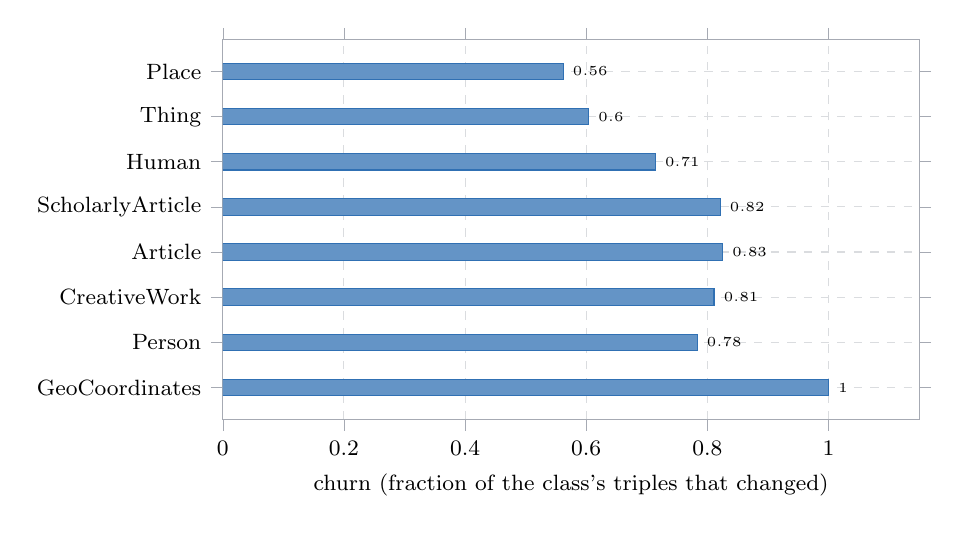
\begin{tikzpicture}
    \begin{axis}[
      kgaxis, xbar, area legend, width=.86\linewidth, height=6.4cm,
      xlabel={churn (fraction of the class's triples that changed)},
      symbolic y coords={GeoCoordinates,Person,CreativeWork,Article,
                         ScholarlyArticle,Human,Thing,Place},
      ytick=data, xmin=0, xmax=1.15,
      bar width=6pt, enlarge y limits=0.1,
      nodes near coords, every node near coord/.append style={font=\tiny,
        /pgf/number format/fixed, /pgf/number format/precision=2},
      ]
      \addplot[fill=kgblue!75, draw=kgblue] coordinates
        {(1.000,GeoCoordinates) (0.825,Article) (0.821,ScholarlyArticle)
         (0.811,CreativeWork) (0.783,Person) (0.714,Human) (0.604,Thing)
         (0.562,Place)};
    \end{axis}
  \end{tikzpicture}
  \caption[\entrydesc{Per-class churn, YAGO 4 to 4.5.0.2}{Share of each class's triples that changed between the two releases}]{Churn per class between YAGO~4 and
    YAGO~4.5.0.2, from metric~9. A value of 1.0 means every triple of the class
    changed. \texttt{GeoCoordinates} was removed outright.}
  \label{fig:churn}
\end{figure}

Metric~10 reports the composition of the change directly.
Table~\ref{tab:diffcomposition} gives added, deleted and unchanged counts inside
a 50{,}000-subject window scoped to \texttt{Person}.

\begin{table}[htbp]
  \centering
  \caption[\entrydesc{Triple diff composition}{Added, deleted and unchanged triples in a Person subject window}]{Added, deleted and unchanged triples inside a
    50{,}000-subject window scoped to \texttt{Person}, from metric~10. Churn is
    $(\text{added} + \text{deleted}) / |T(v_1)|$.}
  \label{tab:diffcomposition}
  \footnotesize
  \pgfplotstabletypeset[
    col sep=comma, string type,
    columns={pair,added,deleted,unchanged,churn},
    columns/pair/.style={column name=Pair, column type=l},
    columns/added/.style={column name=Added, column type=r},
    columns/deleted/.style={column name=Deleted, column type=r},
    columns/unchanged/.style={column name=Unchanged, column type=r},
    columns/churn/.style={column name=Churn, column type=r},
    every head row/.style={before row=\toprule, after row=\midrule},
    every last row/.style={after row=\bottomrule},
  ]{data/diff_composition.csv}
\end{table}

\paragraph{Trajectories (metric~11)} Figure~\ref{fig:trajectories} follows
four graph-level quantities across each series, every one indexed to the first
release of its graph, so a value of 2 means doubled and 0.5 means halved.

\newcommand{\trajpanel}[3]{%
  \begin{axis}[
    kgaxis, scale only axis, width=5.2cm, height=4.6cm, title={#2},
    ymode=log, log basis y=10, ymin=#3, ymax=60,
    ylabel={relative to first release}, ylabel style={font=\scriptsize},
    xtick=data, table/col sep=comma, xticklabels from table={#1}{snapshot},
    x tick label style={font=\scriptsize, rotate=25, anchor=north east},
    enlarge x limits=0.08, legend columns=2,
    legend style={at={(0.5,-0.36)}, anchor=north, font=\scriptsize},
    line legend,
  ]
    \addplot[thick, color=kgnavy, mark=*] table[x expr=\coordindex, y=triples_idx]{#1};
    \addplot[thick, color=kgblue, mark=square*] table[x expr=\coordindex, y=typed_entities_idx]{#1};
    \addplot[thick, color=kgred, mark=triangle*] table[x expr=\coordindex, y=classes_idx]{#1};
    \addplot[thick, color=kggrey, mark=diamond*] table[x expr=\coordindex, y=predicates_idx]{#1};
    \legend{triples, typed entities, classes, predicates}
  \end{axis}}

\begin{figure}[htbp]
  \centering
  \begin{tikzpicture}\trajpanel{data/traj_yago.csv}{YAGO}{0.01}\end{tikzpicture}\hfill
  \begin{tikzpicture}\trajpanel{data/traj_dbpedia.csv}{DBpedia}{0.01}\end{tikzpicture}
  \caption[\entrydesc{Graph-level trajectories}{Triples, entities, classes and predicates across each release series}]{Graph-level
    trajectories from metric~11, each quantity divided by its value in the first
    release of the series, on a logarithmic axis. YAGO's class count falls by a
    factor of 47 at the schema.org rewrite and recovers by a factor of 12;
    DBpedia's classes and predicates stay nearly flat while its typed entities
    grow sixfold.}
  \label{fig:trajectories}
\end{figure}

The two graphs trace different shapes. YAGO grows by a factor of 34 in triples
from YAGO~3 to YAGO~4, from 73 million to 2.49 billion, then loses almost half
at YAGO~4.5. Its class count moves the other way at both steps: from 475{,}673 to
10{,}103 when WordNet synsets gave way to schema.org, then up to 118{,}303 when
YAGO~4.5 imported the Wikidata taxonomy. DBpedia changes gradually by comparison.
Its classes stay between 740 and 772 across the decade and its predicates fall
by 11\%, while its triples double. The one abrupt move is the sixfold growth in
typed entities, most of it between 2022 and 2025, which is the image and
document metadata discussed in Section~\ref{sec:exp1}. A single pair of releases
would show either graph's change as one number; the trajectory shows whether
that change was a step or a drift.

\subsection{Discussion}

The two graphs evolve in opposite directions, and Table~\ref{tab:vocab} makes the
contrast sharp enough to state as a rule.

YAGO churns its classes and holds its predicates. It added 111{,}122 classes
while keeping 7{,}181, a class vocabulary that is 94\% new, and over the same
interval it kept 72 predicates, added 51 and removed 85. The removed predicates
name the cause exactly: \texttt{bioChemInteraction},
\texttt{encodesBioChemEntity}, \texttt{expressedIn}, \texttt{hasMolecularFunction}
and \texttt{inChI} all belong to the biochemical vocabulary, and the removed
classes include \texttt{BioChemEntity}, \texttt{ChemicalSubstance},
\texttt{Gene}, \texttt{MolecularEntity} and \texttt{Protein}. YAGO~4.5 dropped
the life-sciences branch and replaced the class hierarchy with fine-grained
Wikidata classes such as \texttt{Taxon}.

DBpedia does the reverse. It kept 700 of 740 classes over a decade, adding 71 and
removing 40, while its predicates churned violently: 23{,}897 added, 30{,}788
removed, 31{,}036 kept. A hand-maintained ontology stays stable while the
infobox-derived predicate set moves under it. A single year, 2015 to 2016, already
adds 6{,}047 predicates and removes 7{,}347 while the classes barely move, seven
added and one removed. The intermediate release shows when the bulk happened: between 2015 and 2022 DBpedia added 20{,}584 predicates and
removed 27{,}717, while between 2022 and 2025 it added 8{,}102 and removed
7{,}860, and its classes barely moved at all, seven added and eight removed. The
predicate churn is concentrated in the first seven years, the same shape
Table~\ref{tab:churnseries} shows for triples. This is the structural consequence
of DBpedia's extraction process~\cite{bizer2009dbpedia}, and it means the two
graphs need different change metrics to be understood. Watching DBpedia's classes
would show almost nothing; watching YAGO's predicates would show almost nothing.

Figure~\ref{fig:churn} localises YAGO's change. \texttt{GeoCoordinates} reaches
churn 1.0 with 25{,}303 deletions and zero additions, which is removal rather
than revision. \texttt{Article} and \texttt{ScholarlyArticle} sit at 0.825 and
0.821, and their diffs are almost entirely deletions: \texttt{Article} shows 17
additions against 758{,}368 deletions. That single line explains most of the
1.18 billion triple drop between YAGO~4 and YAGO~4.5 seen in
Table~\ref{tab:datasets}. The bulk scholarly-article content left.

\texttt{Person} behaves differently, with 223{,}227 additions against 245{,}398
deletions. Roughly balanced churn at high volume is revision, not removal, and it
is the signature an analyst should look for when asking whether a class was
rewritten or retired. Distinguishing those two cases is exactly what a
churn number alone cannot do and what the added/deleted split in
Table~\ref{tab:diffcomposition} provides.

The DBpedia churn of 2.196 in Table~\ref{tab:diffcomposition} exceeds 1.0, which
is not an error. Churn normalises by $|T_t(v_1)|$, so a class that more than
doubles its triples can exceed unity. DBpedia's \texttt{Person} window grew from
339{,}728 to 784{,}889 triples across the decade. Reading churn above 1.0 as a
bug would be a natural mistake, and the metric definition in
Section~\ref{subsec:churn_metric} is deliberate about the denominator.

Table~\ref{tab:churnseries} splits DBpedia's decade into its release steps,
using metric~9 over the same 50{,}000-subject window.

\begin{table}[htbp]
  \centering
  \caption[\entrydesc{DBpedia churn by release step}{Churn of Thing and Person across the DBpedia releases}]{Churn for \texttt{owl:Thing} and
    \texttt{dbo:Person} across each DBpedia release step, from metric~9, with
    the added and deleted triples for \texttt{dbo:Person}. Each row divides by
    the class's triples in its own earlier release.}
  \label{tab:churnseries}
  \footnotesize
  \pgfplotstabletypeset[
    col sep=comma, string type,
    columns={step,thing,person,person_added,person_deleted},
    columns/step/.style={column name=Step, column type=l},
    columns/thing/.style={column name=\texttt{Thing}, column type=r},
    columns/person/.style={column name=\texttt{Person}, column type=r},
    columns/person_added/.style={column name=\texttt{Person} added, column type=r},
    columns/person_deleted/.style={column name=\texttt{Person} deleted, column type=r},
    every head row/.style={before row=\toprule, after row=\midrule},
    every last row/.style={after row=\bottomrule},
  ]{data/churn_series.csv}
\end{table}

The steps are uneven. Churn for \texttt{Thing} is 2.290 between 2015 and 2022
and 0.746 between 2022 and 2025, and \texttt{Person} follows the same shape at
1.670 and 0.540. Most of the decade's change happened in the first seven years,
and the last three were comparatively quiet. The 2015 to 2016 row gives the
scale of one year of ordinary drift, 0.280 for \texttt{Person}. The steps do not
sum to the decade figure, and they should not: churn divides by the class's
triples in the earlier release, and each step starts from a different release.

Metric~10, run separately over the same two new steps, returns the same
\texttt{Person} churn to four decimal places, 1.670 and 0.540. This is not an
independent check of correctness: metric~9 reuses metric~10's windowing and
diff code, so agreement is expected by construction. It does confirm the
reproducibility that Section~\ref{subsec:protocol} assumes, since the two runs
fetched their triples from live endpoints at different times and still returned
identical sets.

One detail of method affects this table. The 2022 to 2025 comparison was run
over twelve classes rather than eight, because in DBpedia 2022 the four aliases
of \texttt{Person} rank ninth to twelfth by population, and an eight-class run
measures \texttt{Thing}, \texttt{TimePeriod} and \texttt{Species} but omits
people entirely.

One negative result belongs here. YAGO~3 to YAGO~4 cannot be compared per class
at all. The two releases share no class names, because YAGO~3 types entities
against WordNet synsets and Wikipedia categories while YAGO~4 uses schema.org.
The metric~10 run over that pair reports 56{,}021 additions and zero deletions,
arithmetically correct and semantically empty, because the subject window lands
in disjoint identifier spaces. The tooling reports this rather than hiding it,
and Section~\ref{sec:limitations} records it as a limitation. The aggregate
metrics still work, and metric~12 measures the replacement directly. Of YAGO~3's
475{,}673 classes, none survives into YAGO~4: all 475{,}673 are removed and all
10{,}103 of YAGO~4's are new (Table~\ref{tab:vocab}). The predicate vocabulary
is replaced almost as thoroughly, with 4 predicates kept, 77 removed and 153
added. Two consecutive releases of one knowledge graph that share no class at all
is the clearest case of evolution in this thesis, and it is visible only to a
metric that compares whole vocabularies; every per-class metric sees nothing to
compare.

\section{Experiment 3: Efficiency of the Triple Diff}
\label{sec:exp3}

\subsection{Objective and Methodology}

This experiment answers RQ3. Two implementations of the same set difference were
run on identical inputs: a naive version holding triples as strings in a hash
set, and the integer-encoded version of
Section~\ref{subsec:integer_encoding}. Both paths run inside the same invocation and
the implementation asserts that they produce identical results, so the speedup
cannot drift away from being correct while the outputs silently diverge.

Wall-clock time and peak working-set size were recorded for both paths across
five version pairs of different sizes.

\subsection{Results}

Table~\ref{tab:benchmark} reports the measurements.
Figure~\ref{fig:benchmark} plots the time and memory columns.

\begin{table}[htbp]
  \centering
  \caption[\entrydesc{Triple diff benchmark}{Run time and memory of integer-encoded against string sets}]{Integer-encoded against string-based set
    difference on identical inputs. Both paths were asserted to return the same
    added and deleted sets.}
  \label{tab:benchmark}
  \footnotesize
  \pgfplotstabletypeset[
    col sep=comma, string type,
    columns={pair,triples,enc_ms,naive_ms,enc_mb,naive_mb,speedup,memfactor},
    columns/pair/.style={column name=Pair, column type=l},
    columns/triples/.style={column name=Triples, column type=r},
    columns/enc_ms/.style={column name={Enc.\,ms}, column type=r},
    columns/naive_ms/.style={column name={Naive\,ms}, column type=r},
    columns/enc_mb/.style={column name={Enc.\,MB}, column type=r},
    columns/naive_mb/.style={column name={Naive\,MB}, column type=r},
    columns/speedup/.style={column name=Time, column type=r},
    columns/memfactor/.style={column name=Memory, column type=r},
    every head row/.style={before row=\toprule, after row=\midrule},
    every last row/.style={after row=\bottomrule},
  ]{data/diff_benchmark.csv}
\end{table}

\begin{figure}[htbp]
  \centering
  \begin{tikzpicture}
    \begin{axis}[
      kgaxis, ybar, area legend, width=.49\linewidth, height=5.6cm,
      name=timeplot,
      xtick=data, xticklabels={DBp15/16,DBp15/22,DBp22/25,DBp15/25,YAGO4/4.5},
      x tick label style={font=\tiny, rotate=35, anchor=east},
      ymin=0, bar width=5pt, enlarge x limits=0.12,
      title={wall-clock time (ms)},
      legend style={font=\scriptsize, at={(0.03,0.97)}, anchor=north west},
      ]
      \addplot[fill=kgblue!75, draw=kgblue] table[col sep=comma,
        x expr=\coordindex, y=enc_ms]{data/diff_benchmark.csv};
      \addplot[fill=kggrey!50, draw=kggrey] table[col sep=comma,
        x expr=\coordindex, y=naive_ms]{data/diff_benchmark.csv};
      \legend{encoded, naive}
    \end{axis}
    \begin{axis}[
      kgaxis, ybar, area legend, width=.49\linewidth, height=5.6cm,
      at={(timeplot.south east)}, xshift=0.9cm, anchor=south west,
      xtick=data, xticklabels={DBp15/16,DBp15/22,DBp22/25,DBp15/25,YAGO4/4.5},
      x tick label style={font=\tiny, rotate=35, anchor=east},
      ymin=0, bar width=5pt, enlarge x limits=0.12,
      title={peak working set (MB)},
      legend style={font=\scriptsize, at={(0.03,0.97)}, anchor=north west},
      ]
      \addplot[fill=kgblue!75, draw=kgblue] table[col sep=comma,
        x expr=\coordindex, y=enc_mb]{data/diff_benchmark.csv};
      \addplot[fill=kggrey!50, draw=kggrey] table[col sep=comma,
        x expr=\coordindex, y=naive_mb]{data/diff_benchmark.csv};
      \legend{encoded, naive}
    \end{axis}
      \end{tikzpicture}
  \caption[\entrydesc{Triple diff benchmark}{Speed-up and memory saving of the integer encoding}]{Integer encoding against the string baseline.
    Time improves by a factor between 2.3 and 6.2; memory improves by a factor
    between 16 and 19, and the memory result is the one that decides whether the
    comparison runs at all on a 16\,GB client.}
  \label{fig:benchmark}
\end{figure}

\subsection{Discussion}

The memory result matters more than the speed result, and it is worth being
precise about why.

Peak working set falls by a factor of 16 to 19 across all five pairs, from
318.8\,MB to 16.5\,MB on the smallest DBpedia step and from 574.7\,MB to
35.3\,MB on the YAGO pair. A triple stored as
three strings costs roughly 200 bytes with allocator overhead and pointer
indirection; the same triple encoded as three 32-bit integers costs 12 bytes in a
packed array. Hashing is then an integer operation over a contiguous buffer
rather than a string comparison chasing pointers, which is where the time saving
comes from as a side effect.

On a 16\,GB client the difference decides feasibility rather than comfort.
Extrapolating the naive path's 575\,MB for three million triples to a
hundred-million-triple comparison gives roughly 19\,GB, which does not fit. The
encoded path's 35\,MB extrapolates to roughly 1.2\,GB, which does.

The speedup varies from 2.34 to 6.17, and the variation is informative rather
than noise. The YAGO pair shows the smallest speedup on the largest input, which
looks backwards until the composition in Table~\ref{tab:diffcomposition} is taken
into account: that pair has the highest proportion of triples present in both
versions, 445{,}462 unchanged. Unchanged triples are the case where both
implementations do the same amount of work, because the hash lookup succeeds in
both and the string path avoids the allocation that dominates its cost elsewhere.
The encoding wins most where the sets differ most, which is exactly where a
version diff is doing useful work.

Reporting the benchmark across five pairs rather than one avoids a claim the
data would not support. A single measurement would have given 6.17 and implied
it was the number; the range 2.34 to 6.17 is the honest result, and the
mechanism above explains the spread.

Fernández et al.~\cite{fernandez2015dbpedia} use integer encoding in the DBpedia
Wayback Machine over prepared archives. The contribution here is pairing it with
the subject-window scoping of Section~\ref{subsec:subject_window}, which is what removes
the global sort and lets the same idea run against a live endpoint.

\section{Experiment 4: Entropy-Weighted against Classic PageRank}
\label{sec:exp4}

\subsection{Objective and Methodology}

This experiment evaluates the variant proposed in
Section~\ref{sec:entropy_weighted_pagerank}. Both rankings were computed over the
same edge set, sampled by breadth-first expansion from 50 InfoRank seeds to a
budget of 200{,}000 edges, which yielded 5{,}372 nodes and 11{,}558 edges over 27
distinct predicates in YAGO~4. Damping was 0.85 and the convergence tolerance
$10^{-9}$, with a cap of 100 iterations.

\subsection{Results}

Table~\ref{tab:weights} reports the extreme predicate weights.
Figure~\ref{fig:weights} plots them.

\begin{table}[htbp]
  \centering
  \caption[\entrydesc{Predicate weights}{Most and least informative predicates on the YAGO 4 sample}]{Highest and lowest normalised property-entropy
    weights $w(p)$ on the sampled YAGO~4 subgraph, from metric~7.}
  \label{tab:weights}
  \footnotesize
  \begin{tabular}{lr@{\hskip 2cm}lr}
    \toprule
    Predicate & $w(p)$ & Predicate & $w(p)$ \\
    \midrule
    \texttt{geo}           & 1.000 & \texttt{nationality}    & 0.261 \\
    \texttt{image}         & 0.948 & \texttt{knowsLanguage}  & 0.191 \\
    \texttt{containsPlace} & 0.881 & \texttt{sport}          & 0.174 \\
    \texttt{children}      & 0.863 & \texttt{gender}         & 0.034 \\
    \bottomrule
  \end{tabular}
\end{table}

\begin{figure}[htbp]
  \centering
  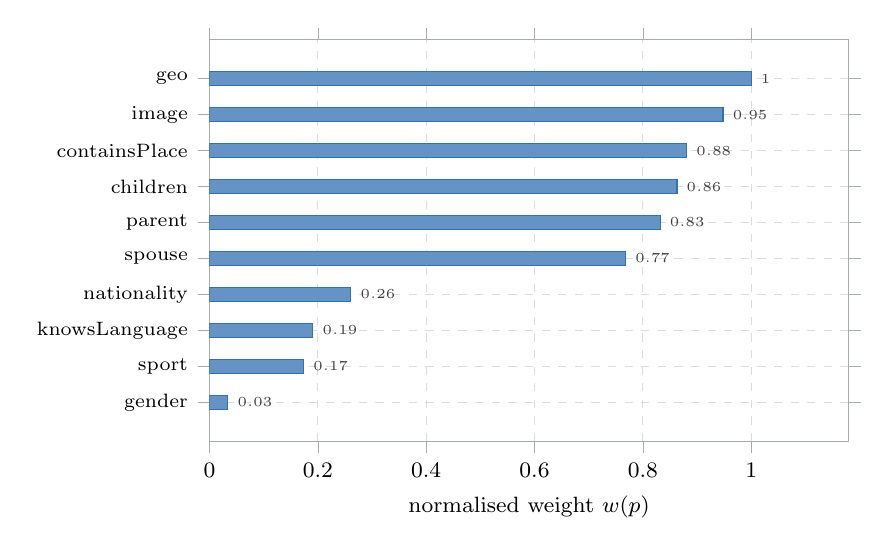
\begin{tikzpicture}
    \begin{axis}[
      kgbar, width=.8\linewidth, height=6cm,
      xlabel={normalised weight $w(p)$}, xmax=1.18,
      symbolic y coords={gender,sport,knowsLanguage,nationality,spouse,parent,
                         children,containsPlace,image,geo},
      ]
      \addplot[fill=kgblue!75, draw=kgblue] coordinates
        {(1.000,geo) (0.948,image) (0.881,containsPlace) (0.863,children)
         (0.832,parent) (0.768,spouse) (0.261,nationality) (0.191,knowsLanguage)
         (0.174,sport) (0.034,gender)};
    \end{axis}
  \end{tikzpicture}
  \caption[\entrydesc{Predicate weights in entropy-weighted PageRank}{The edge weight each predicate receives in the PageRank walk}]{Normalised property
    entropy per predicate on the sampled YAGO~4 subgraph. The weight spans a
    factor of 29 between \texttt{geo} and \texttt{gender}, which is the
    separation classic PageRank cannot express.}
  \label{fig:weights}
\end{figure}

The weighted variant converged in 43 iterations with a mean delta of
$9.0 \times 10^{-10}$. The unweighted baseline did not converge within the
100-iteration cap, finishing at a mean delta of $2.8 \times 10^{-9}$. Of the
5{,}372 nodes, 5{,}327 changed rank, which is 99.2\%.

\subsection{Discussion}

The weighting changes the ranking substantially rather than perturbing it.
Moving 99.2\% of nodes means this is a different ranking, not a reordering of
ties, and the weight range in Figure~\ref{fig:weights} explains why: an edge
labelled \texttt{geo} carries 29 times the weight of one labelled
\texttt{gender}. In classic PageRank both contribute identically, so an entity
connected to many others by gender accumulates the same importance as one
connected by coordinates.

The convergence result was not anticipated and deserves care, because it is
tempting to over-claim it. The weighted walk converged in 43 iterations where the
unweighted one did not converge in 100. A plausible mechanism is that
down-weighting high-volume, low-entropy predicates such as
\texttt{gender} removes the dense near-uniform subgraphs those predicates create,
and dense uniform structure is what slows a power iteration. That explanation
fits the data but this experiment does not establish it: one sampled subgraph of
one snapshot is not enough to claim a general convergence advantage, and the
honest statement is that the weighted variant converged here and the unweighted
one did not.

The comparison against Menendez et al.~\cite{menendez2018ranking} is
direct. They decouple ranking from raw degree by ranking on information content
at the node level. Entropy-weighted PageRank pushes the same idea into the edge
weights, so information affects not only which nodes score highly but how score
flows between them. Neither approach subsumes the other, and metric~5 in this
thesis implements theirs as the node-level counterpart.

The sampling is a real constraint on this result. Full-graph PageRank over 2.5
billion triples is out of reach on the client hardware of
Table~\ref{tab:machines}, so metric~7 seeds from the InfoRank results of metric~5
and expands breadth-first. Seeding from the most informative entities rather than
uniformly at random keeps the sample connected. An earlier implementation took
an unordered \texttt{LIMIT} instead, which returned a star forest with almost no
edges between sampled nodes and made PageRank meaningless on it. That failure is
worth recording because the resulting numbers looked plausible.

\section{Experiment 5: Cross-Graph Comparison}
\label{sec:exp5}

\subsection{Objective and Methodology}

The final experiment answers RQ4 by applying the class-level metrics across two
different knowledge graphs rather than two versions of one. Metric~13 matched
classes between YAGO~4.5.0.2 and DBpedia 2025-12-01 by local name and computed
population, predicate count and class entropy on both sides. The matcher was
given the 150 most populated classes of each graph and found sixteen class names
common to both.

The experiment was then repeated against DBpedia 2015-10, 2016 and
2022-12-01. Fifteen or sixteen classes matched in each, which turns the
cross-graph comparison from a single observation into a four-point series
across a decade. YAGO~4.5.0.2 does not change between these runs, so every
movement in that series is on the DBpedia side.

To test whether the results depend on the YAGO release, the whole series was
repeated with YAGO~4 in place of YAGO~4.5.0.2. YAGO~4 matched twenty-three to
twenty-five class names per DBpedia release, and twenty-one to twenty-three of
them were measured. The two left out are its root classes, \texttt{Thing} with
66.9 million entities and \texttt{CreativeWork} with 35.9 million. Both match a
DBpedia class by name, but the entropy histogram over either drove the QLever
server past the 12\,GB of memory on the machine hosting it, and the operating
system killed the process. Every YAGO~4 run excludes the two by name, and each
result file records the exclusion. Little is lost: \texttt{Thing} is the root on
both sides, so its entropy describes the whole graph rather than a concept.

YAGO~3 was run against DBpedia 2015 and matched no class at all, for the reason
given in the discussion below. That reason does not depend on the DBpedia
release, so YAGO~3 was not run against the later three. Nine of the twelve
possible pairings were therefore measured.

Metric~10 is deliberately not used here. YAGO and DBpedia have disjoint subject
IRIs, so a subject window lands inside one graph and reports everything as added:
arithmetically correct, semantically empty. The implementation warns when it
detects this.

\subsection{Results}

Table~\ref{tab:crosskg} reports the sixteen matched classes.
Figure~\ref{fig:crosskg} plots the population and entropy columns.

\begin{table}[htbp]
  \centering
  \caption[\entrydesc{Cross-graph class comparison}{Population, entropy and predicates for sixteen shared classes}]{The sixteen classes matched
    automatically between YAGO~4.5.0.2 and DBpedia 2025-12-01 over the 150 most
    populated classes of each graph, from metric~13.
    $\Delta H$ is YAGO minus DBpedia.}
  \label{tab:crosskg}
  \footnotesize
  \pgfplotstabletypeset[
    col sep=comma, string type,
    columns={class,pop_yago,pop_dbpedia,H_yago,H_dbpedia,delta_H,
             preds_yago,preds_dbpedia},
    columns/class/.style={column name=Class, column type=l},
    columns/pop_yago/.style={column name=YAGO $|E_t|$, column type=r},
    columns/pop_dbpedia/.style={column name=DBp.\ $|E_t|$, column type=r},
    columns/H_yago/.style={column name=$H_{\text{Y}}$, column type=r},
    columns/H_dbpedia/.style={column name=$H_{\text{D}}$, column type=r},
    columns/delta_H/.style={column name=$\Delta H$, column type=r},
    columns/preds_yago/.style={column name=$|P|_{\text{Y}}$, column type=r},
    columns/preds_dbpedia/.style={column name=$|P|_{\text{D}}$, column type=r},
    every head row/.style={before row=\toprule, after row=\midrule},
    every last row/.style={after row=\bottomrule},
  ]{data/cross_kg.csv}
\end{table}

\begin{figure}[htbp]
  \centering
  \begin{tikzpicture}
    \begin{axis}[
      kgaxis, xbar, area legend, width=.78\linewidth, height=11cm,
      y dir=reverse, ytick=data,
      yticklabels={person,politician,mountain,administrativearea,river,album,movie,building,village,writer,stream,organization,ship,road,school,artist},
      yticklabel style={font=\scriptsize},
      xlabel={class entropy (bits)}, xmin=0, xmax=23,
      bar width=3.4pt, enlarge y limits=0.035,
      legend style={at={(0.5,1.02)}, anchor=south, legend columns=2,
                    /tikz/every even column/.append style={column sep=8pt}},
      ]
      \addplot[fill=kggreen!80, draw=kggreen] table[col sep=comma,
        y expr=\coordindex, x=H_yago]{data/cross_kg_plot.csv};
      \addplot[fill=kgolive!80, draw=kgolive] table[col sep=comma,
        y expr=\coordindex, x=H_dbpedia]{data/cross_kg_plot.csv};
      \legend{YAGO 4.5.0.2, DBpedia 2025}
    \end{axis}
  \end{tikzpicture}
  \caption[\entrydesc{Cross-graph class entropy}{YAGO 4.5.0.2 against DBpedia 2025 entropy per matched class}]{Class entropy for the sixteen matched
    classes. YAGO reports higher entropy everywhere except
    \texttt{organization}, where the two graphs agree to within 0.001 bits.}
  \label{fig:crosskg}
\end{figure}

Table~\ref{tab:crosskgseries} holds the YAGO side fixed and varies the DBpedia
release, so the last four columns trace how far apart the two graphs were at
each point of the decade.

\begin{table}[htbp]
  \centering
  \caption[\entrydesc{Cross-graph comparison across a decade}{Entropy gap between YAGO 4.5.0.2 and four DBpedia releases}]{The same comparison run
    against four DBpedia releases with YAGO~4.5.0.2 fixed on the other side,
    for the fifteen classes matched in all four. All values are object entropy
    in bits; the final columns give
    $|H_{\text{YAGO}} - H_{\text{DBpedia}}|$ per release.}
  \label{tab:crosskgseries}
  \footnotesize
  \pgfplotstabletypeset[
    col sep=comma, string type,
    columns={class,H_yago,H_2015,H_2016,H_2022,H_2025,gap2015,gap2016,gap2022,gap2025},
    columns/class/.style={column name=Class, column type=l},
    columns/H_yago/.style={column name=$H_{\text{Y}}$, column type=r},
    columns/H_2015/.style={column name=2015, column type=r},
    columns/H_2016/.style={column name=2016, column type=r},
    columns/H_2022/.style={column name=2022, column type=r},
    columns/H_2025/.style={column name=2025, column type=r},
    columns/gap2015/.style={column name=gap 15, column type=r},
    columns/gap2016/.style={column name=gap 16, column type=r},
    columns/gap2022/.style={column name=gap 22, column type=r},
    columns/gap2025/.style={column name=gap 25, column type=r},
    every head row/.style={before row=\toprule, after row=\midrule},
    every last row/.style={after row=\bottomrule},
  ]{data/crosskg_series.csv}
\end{table}

Table~\ref{tab:crosskgseriesyago4} repeats the series with YAGO~4 on the YAGO
side. The DBpedia columns agree with Table~\ref{tab:crosskgseries} wherever the
two share a class, as they must, since the DBpedia classes are the same; only
the YAGO value and therefore the gap differ.

\begin{table}[htbp]
  \centering
  \caption[\entrydesc{Cross-graph comparison against YAGO 4}{The same series with YAGO 4, as a control}]{The series of
    Table~\ref{tab:crosskgseries} with YAGO~4 in place of YAGO~4.5.0.2, for the
    nineteen classes matched against all four DBpedia releases. YAGO~4's root
    classes \texttt{Thing} and \texttt{CreativeWork} are excluded; see the text.
    Object entropy in bits; the final columns give
    $|H_{\text{YAGO}} - H_{\text{DBpedia}}|$ per release.}
  \label{tab:crosskgseriesyago4}
  \footnotesize
  \setlength{\tabcolsep}{4.5pt}
  \pgfplotstabletypeset[
    col sep=comma, string type,
    columns={class,H_yago,H_2015,H_2016,H_2022,H_2025,gap2015,gap2016,gap2022,gap2025},
    columns/class/.style={column name=Class, column type=l},
    columns/H_yago/.style={column name=$H_{\text{Y4}}$, column type=r},
    columns/H_2015/.style={column name=2015, column type=r},
    columns/H_2016/.style={column name=2016, column type=r},
    columns/H_2022/.style={column name=2022, column type=r},
    columns/H_2025/.style={column name=2025, column type=r},
    columns/gap2015/.style={column name=gap 15, column type=r},
    columns/gap2016/.style={column name=gap 16, column type=r},
    columns/gap2022/.style={column name=gap 22, column type=r},
    columns/gap2025/.style={column name=gap 25, column type=r},
    every head row/.style={before row=\toprule, after row=\midrule},
    every last row/.style={after row=\bottomrule},
  ]{data/crosskg_series_yago4.csv}
\end{table}

Figure~\ref{fig:crosskggaps} plots the gap columns of both tables, one row per
class and one marker per DBpedia release, so a row whose markers spread apart is
a class whose distance to DBpedia moved, and a marker at zero is agreement.

\begin{figure}[htbp]
  \centering
  \begin{tikzpicture}
    \figgapdots{data/crosskg_series.csv}{against YAGO 4.5.0.2}{6.3cm}
  \end{tikzpicture}\hfill
  \begin{tikzpicture}
    \figgapdots{data/crosskg_series_yago4.csv}{against YAGO 4}{8cm}
  \end{tikzpicture}
  \caption[\entrydesc{Cross-graph entropy gap per DBpedia release}{Gap per class and release for both YAGO versions}]{The entropy gap between
    YAGO and each DBpedia release, per class, from
    Tables~\ref{tab:crosskgseries} (left) and~\ref{tab:crosskgseriesyago4}
    (right). The 2016 markers (squares) sit furthest right on almost every row,
    the release-wide dip discussed below. \texttt{Organization} reaches zero
    only on the left, against DBpedia 2025; on the right it stays between 4.5
    and 5.9 bits.}
  \label{fig:crosskggaps}
\end{figure}

\subsection{Discussion}

Two findings come out of Table~\ref{tab:crosskg}, and the second is the more
interesting.

The first is the predicate-count asymmetry, which holds across all sixteen
classes without exception. DBpedia uses 3{,}025 distinct predicates on
\texttt{building} where YAGO uses 31, 2{,}888 on \texttt{administrativearea}
where YAGO uses 34, 1{,}315 on \texttt{mountain} where YAGO uses 24. The ratio
ranges from 24 to 92 and never falls below an order of magnitude. This is the
curated against extracted contrast of Table~\ref{tab:datasets} reproduced at
class granularity, and sixteen consecutive confirmations make it structural
rather than an artefact of the graph-level totals.

Class entropy follows the same direction. YAGO reports higher object entropy than
DBpedia on fifteen of the sixteen classes, with margins from 1.05 bits on
\texttt{ship} to 7.84 bits on \texttt{writer}. The exception is the one
discussed below. The direction depends on the YAGO release, though not
strongly. YAGO~4 sits closer to DBpedia overall, with a mean gap of 2.42 to 3.31
bits across the four releases against 3.71 to 4.89 for YAGO~4.5, and it falls
below DBpedia on \texttt{ship} in every release and on \texttt{building},
\texttt{road} and \texttt{sportsevent} in at least one.

The second is \texttt{organization}, and widening the scan made it more
interesting rather than less. It remains the only class where the entropies
agree: 14.2752 bits in YAGO against 14.2754 in DBpedia, a difference of 0.0002
bits, while the populations differ by a factor of 3.7 in DBpedia's favour,
383{,}356 against 103{,}600. Two independently built knowledge graphs, one
curated from Wikidata and one extracted from infoboxes, describe organisations
with the same amount of information per entity.

The deeper scan removed the explanation I first reached for. At eight classes
\texttt{organization} was the only one where DBpedia held more entities, which
made size inversion and entropy agreement look like a single phenomenon. At
sixteen classes \texttt{artist} is also larger in DBpedia, 113{,}477 against
49{,}271, and its entropies differ by 4.09 bits. The two properties are
independent, and whatever makes organisations agree is not that DBpedia has more
of them.

The four-release series settles what a single pairing could not, and it
contradicts the reading I first gave this result. The gap does not close
gradually. Against DBpedia 2015, 2016 and 2022 it stays between 0.63 and 0.72
bits, and against 2025 it is 0.0001: level across seven years, then gone.
DBpedia's own value is not level over that span. It is 14.908 bits in 2015,
drops below YAGO's to 13.560 in 2016, returns to 14.929 in 2022, and reaches
14.2754 in 2025, against a YAGO value of 14.2752 that is fixed in this series. What stays
level is the distance, and what happens in 2025 is that the distance vanishes.
This is a discontinuity between two consecutive releases, not a decade of
convergence, and no explanation built on gradual coverage improvement survives
it.

A discontinuity points at a change in how the class is built rather than at how
much of it there is. The population grows smoothly across the same four
releases, 267{,}318, 286{,}482, 352{,}131 and 383{,}356, so the collapse is not
a sampling effect of a suddenly larger class. YAGO~4.5 draws its classes from
Wikidata, and the simplest hypothesis consistent with the shape is that DBpedia
2025 began deriving organisation descriptions from the same upstream source, in
which case both graphs would inherit one value distribution and therefore one
entropy. This thesis does not test that hypothesis. What it does establish is
that the agreement appeared between 2022 and 2025 and not before, which is a far
narrower claim to check than convergence over a decade.

The YAGO~4 control changes how the result reads. Against YAGO~4,
\texttt{organization} is an ordinary class: the gap is 4.56, 5.91, 4.54 and 5.19
bits across the four DBpedia releases (Table~\ref{tab:crosskgseriesyago4}), the
same order as \texttt{movie} or \texttt{place}. The agreement therefore exists
only between YAGO~4.5.0.2 and DBpedia 2025, and it needed both graphs to move.
YAGO's own \texttt{Organization} changed more between its two releases than any
other class the two series share. It shrank from 2{,}144{,}509 entities to
103{,}600, and its entropy fell by 5.19 bits, from 19.47 to 14.28. DBpedia moved
0.65 bits between 2022 and 2025. Two independent changes, one in each graph,
arrived at the same value to within 0.0002 bits. This weakens the shared-source
hypothesis, because YAGO~4 was built from Wikidata as well and never came close.
It makes coincidence more plausible, though not enough to settle the question.

Table~\ref{tab:crosskgseries} also rules out any general convergence, and the
2016 release shows why a single step can mislead. Between 2015 and 2016 the gap
widens for every one of the fifteen classes, and between 2016 and 2022 it narrows
for every one. A shift shared by all fifteen classes is a property of the 2016
release rather than of any class in it, and Table~\ref{tab:datasets} is
consistent with that: the 2016 matched subset is 16\% smaller than 2015's,
142{,}764{,}052 triples against 169{,}621{,}442. The YAGO~4 series repeats the
pattern: sixteen of its nineteen classes widen between 2015 and 2016, and
eighteen narrow between 2016 and 2022. The shift now appears against two
different YAGO releases, which places it in DBpedia 2016 itself. Taken across the decade, the
graphs end further apart on nine of the fifteen classes, and seven of them widen
at each of the 2015, 2022 and 2025 releases, among them \texttt{writer} at
6.418, 7.606 and 7.839 bits and \texttt{person} at 5.347, 6.083 and 6.494. Against YAGO~4 the graphs end further apart on twelve of nineteen classes. The
graphs are drifting apart on most of what they share, which makes
\texttt{organization} an exception against a trend rather than the leading edge
of one.

I did not expect this result and I remain wary of it. Landing within 0.0001 bits
is too precise to call coincidence, and one class on four time points is too
thin to call a mechanism. I report the shape as a measurement and the Wikidata
hypothesis as the obvious thing to test next; Section~\ref{sec:future_work}
says how.

Four facts about the scope of this experiment belong in the results rather
than in a footnote, because they bound what the table supports.

First, the YAGO~4 control is incomplete by two classes. \texttt{Thing} and
\texttt{CreativeWork} are excluded from every YAGO~4 run because the server
cannot hold their entropy histograms, so Table~\ref{tab:crosskgseriesyago4}
covers the nineteen classes below them. Section~\ref{sec:limitations} records
this.

Second, each pairing covers fifteen or sixteen classes, not the 150 candidates
the matcher scanned on each side. Name matching succeeds only where both graphs
happen to use the same local name for a class, and across a curated schema.org
vocabulary and an infobox-derived one that is the exception rather than the
rule. Sixteen matches is therefore the honest yield of an automatic method, and a
larger comparison would need instance-level alignment rather than a longer
candidate list.

Third, the method fails completely against YAGO~3, and it fails in a way worth
measuring rather than asserting. Metric~13 run with YAGO~3 against DBpedia
2015, the one pairing whose two releases date from the same year, returns
\emph{zero} matched classes. This is not a
shortage of overlap but a structural impossibility: every YAGO~3 class is named
\texttt{wordnet\_<name>\_<synsetid>} or \texttt{wikicat\_<name>}, so its local
name carries a prefix and, for the WordNet branch, a nine-digit synset
identifier. The class holding 180{,}599 people is
\texttt{wordnet\_person\_100007846}, which is not equal to \texttt{Person} under
any exact comparison, at any scan depth. By contrast YAGO~4 and YAGO~4.5 adopted
schema.org names and match twenty-three and sixteen DBpedia 2025 classes
respectively. Name matching therefore survives a vocabulary extension and does
not survive an ontology rewrite, which is a property of the method rather than
of these particular graphs.

Fourth, DBpedia models \texttt{Person} four times over. Its 2025 release carries
\texttt{dbo:Person} with 2{,}125{,}575 entities, \texttt{schema:Person} with
2{,}125{,}571, \texttt{dul:NaturalPerson} with 2{,}125{,}572 and
\texttt{foaf:Person} with 2{,}125{,}569: four aliases of one class, spanning six
entities in total. Metric~13 matched YAGO's \texttt{schema:Person} against
\texttt{foaf:Person}, and the choice among the four was arbitrary. The numbers
are robust to it, since the aliases differ by 0.0003\%, but the arbitrariness is
a property of name matching that a reader should know about. A graph that
maintained genuinely different classes under one local name would not be so
forgiving, and nothing in the method would detect the difference.

The limitation here is real and worth stating plainly rather than burying in
Chapter~\ref{chap:conclusion}. Classes are matched by local name at the schema
level, not by instance-level \texttt{owl:sameAs} linkage. So
\texttt{schema:Person} in YAGO and \texttt{dbo:Person} in DBpedia are treated as
the same class because their local names agree, without any check that they
contain the same entities or model the concept the same way. Ringler and
Paulheim~\cite{ringler2017one} show these graphs are not interchangeable, so the
assumption is known to be imperfect. Name matching is what makes the comparison
automatic and repeatable across sixteen classes instead of manual for one, and that
trade is the right one for a metric, but a $\Delta H$ of 6.49 bits on
\texttt{person} should be read as a difference between two class extents that
share a name, not between two descriptions of the same entities.

The snapshots are also not date-aligned. YAGO~4.5 reflects 2024 data and DBpedia
2025-12-01 reflects a later crawl, so a small part of any difference is elapsed
time rather than design. The predicate-count gap is far too large to be explained
that way, but the population figures should be read with it in mind.

\chapter{Conclusion and Future Work}
\label{chap:conclusion}

\section{Summary}
\label{sec:summary}

This thesis set out to measure how knowledge graphs change between releases, at
a scale where the graphs do not fit in memory. It answers its four questions as
follows.

\textbf{RQ1, can a metric catalogue be computed exactly through a SPARQL
endpoint?} Yes. Thirteen metrics across the class, entity and global level were
implemented in Rust and run against seven snapshots, the largest holding
2{,}489{,}858{,}800 triples. No metric loads the graph. Entropy is the case that
looks impossible at first, because the definition ranges over every object value
of a class, and Section~\ref{subsec:count_of_counts} shows it is not: entropy
depends only on the multiset of value counts, so a nested \texttt{GROUP BY}
folds hundreds of millions of values into a few hundred histogram rows and the
result is exact rather than sampled. The profile the catalogue produces behaves
as the construction of each graph predicts. Labels and \texttt{sameAs} carry the
most information for \texttt{Person}, gender carries almost none, and DBpedia's
predicate entropy exceeds YAGO's on every shared class because DBpedia draws
from 54{,}933 predicates where YAGO draws from 123.

\textbf{RQ2, how do the metrics change between versions, and where does the
change concentrate?} The change concentrates sharply, and the two graphs
concentrate it in opposite places. YAGO replaced 94\% of its class vocabulary
between 4 and 4.5.0.2, adding 111{,}122 classes while keeping 7{,}181, and held
its predicates nearly still at 72 kept. DBpedia did the reverse over a decade,
keeping 700 of 740 classes while 30{,}788 predicates disappeared and 23{,}897
arrived. At class level, metric~9 localises YAGO's change to the content that
left: \texttt{GeoCoordinates} reached churn 1.0 as pure deletion, and
\texttt{Article} recorded 758{,}368 deletions against 17 additions, which
accounts for most of the 1.18 billion triple drop. \texttt{Person} behaved
differently, 223{,}227 added against 245{,}398 deleted, which is revision rather
than retirement. Separating those two cases is what the added and deleted split
provides and a single churn number cannot.

\textbf{RQ3, can version comparison run on commodity hardware?} Yes, and the
integer encoding is what makes it so. Against a string-based baseline on
identical inputs, the encoded path ran 2.34 to 6.17 times faster and held its
working set in 16 to 19 times less memory. The memory result is the one that
decides feasibility: extrapolating the baseline's 575\,MB for three million
triples to a hundred-million-triple comparison gives roughly 19\,GB, which does
not fit on the 16\,GB client, while the encoded path's 35\,MB extrapolates to
about 1.2\,GB, which does. Both paths run inside the same invocation and the
implementation asserts they return identical sets, so the speedup cannot drift
away from being correct.

\textbf{RQ4, what do the metrics say across two different graphs?} They work, and
they report a consistent structural difference. Metric~13 matched sixteen
classes automatically between YAGO~4.5.0.2 and DBpedia 2025 and found DBpedia
using at least an order of magnitude more predicates on every one, with ratios
from 24 to 92: 3{,}025 against 31 on \texttt{building}, 2{,}888 against 34 on
\texttt{administrativearea}, 1{,}315 against 24 on \texttt{mountain}. Sixteen
classes without an exception makes that structural.

The exception is worth more than the rule. \texttt{Organization} is the only
class of the sixteen where the two graphs report the same entropy, 14.2752 bits
against 14.2754. Repeating the comparison against DBpedia 2015, 2016 and 2022
shows the agreement is recent: across those three releases the two graphs sat
between 0.63 and 0.72 bits apart, and the distance vanished only between 2022
and 2025, while YAGO's value never moved. Over the same decade the graphs ended
further apart on nine of the fifteen classes measured in all four releases, so
this is an exception against a trend. Repeating the series with YAGO~4 on the
YAGO side shows the agreement needed both graphs to move: against YAGO~4,
\texttt{organization} stays 4.5 to 5.9 bits from DBpedia in every release,
and YAGO's own value fell by 5.19 bits between its two releases. It is the
single result in this thesis I did not expect, and four time points are not
enough to explain it.

The entropy-weighted PageRank variant of
Section~\ref{sec:entropy_weighted_pagerank} moved 5{,}327 of 5{,}372 sampled
nodes, which makes it a different ranking rather than a reordering of ties. On
the sampled YAGO~4 subgraph it converged in 43 iterations where the unweighted
baseline did not converge in 100.

\section{Limitations}
\label{sec:limitations}

Five limitations constrain these results, and each is a consequence of a design
decision made deliberately rather than an oversight.

\textbf{The triple diff is exact inside a subject window, not over the whole
graph.} Metric~10 takes the lexicographically first $n$ subjects from each side
and cuts both at the smaller bound. Inside that window the result is exact. It
says nothing about subjects outside it. The alternative, sorting both graphs
globally, is what the subject window exists to avoid: QLever asked for 12.7\,GB
to sort a graph far smaller than YAGO and refused the query. Whole-graph windows
on billion-triple graphs are not feasible through SPARQL, and the implementation
says so rather than returning a number that looks complete.

\textbf{The YAGO~4 cross-graph runs leave out two root classes.} YAGO~4's class
distribution is far more top-heavy than YAGO~4.5's: its largest classes are
\texttt{Thing} at 66.9 million entities and \texttt{CreativeWork} at 35.9
million, where YAGO~4.5's largest is \texttt{Taxon} at 3.5 million. Both match
a DBpedia class by name. Counting their predicates became feasible once the
query grouped by predicate instead of asking for \texttt{COUNT(DISTINCT)}, which
had requested 11.1\,GB, but the entropy histogram still pushed the QLever server
past the 12\,GB of the machine hosting it, and the operating system killed it.
Both classes are therefore excluded from every YAGO~4 run, which the result files
record. The loss is small, because a root class measures the whole graph rather
than a concept, but it is a gap that more memory would close. The
\texttt{organization} result also still rests on one class and four time points,
now measured against two YAGO releases.

\textbf{Cross-graph class matching is by local name.} Metric~13 treats
\texttt{schema:Person} and \texttt{dbo:Person} as the same class because the
local names agree. It does not check that they contain the same entities, and where a graph
carries several aliases of one class the choice among them is arbitrary: DBpedia
2025 holds four \texttt{Person} classes within six entities of one another, and
the metric matched one of them without preferring it. The method also yields only
fifteen or sixteen matched classes from 150 candidates per side for YAGO~4.5,
and twenty-three to twenty-five for YAGO~4, because two differently built
vocabularies rarely agree on a local name. Ringler
and Paulheim~\cite{ringler2017one} show these graphs are not interchangeable, so
the assumption is known to be imperfect, and a $\Delta H$ of 6.49 bits on
\texttt{person} compares two class extents that share a name rather than two
descriptions of the same entities.

\textbf{Per-class metrics cover the top classes, not all of them.} A snapshot
with 118{,}303 classes cannot have every class measured at reasonable cost, so
the runs cover the most populated ones. The pinned pass mitigates this for
comparison by fixing the class list, but a change confined to rare classes would
not appear in these results.

\textbf{YAGO~3 cannot be compared per class to YAGO~4 at all.} The two releases
share no class names, because YAGO~3 types entities against WordNet synsets and
Wikipedia categories under a four-layer taxonomy while YAGO~4 uses schema.org. A
per-class comparison would need a hand-built synset mapping and a transitive
\texttt{rdf:type/\allowbreak rdfs:subClassOf*} closure, and without them metric~10 over that
pair reports 56{,}021 additions and zero deletions: correct arithmetic, no
meaning. The aggregate metrics still capture the overhaul, with the class count
falling from 475{,}673 to 10{,}103.

\textbf{Entropy-weighted PageRank normalises by out-degree, not by weight mass.}
Each edge contributes $w(p) \cdot \mathrm{PR}(u) / \mathrm{outdeg}(u)$, so a node
whose edges all carry low weights leaks score rather than redistributing it. The
ranking is still a valid ordering, but it is not a probability distribution in
the way classic PageRank is. The results of Section~\ref{sec:exp4} also come from
a sampled subgraph of 5{,}372 nodes, not the full graph, so the convergence
observation is a single data point and should not be read as a general claim.

\section{Future Work}
\label{sec:future_work}

Four directions follow.

\textbf{More graphs, starting with Wikidata.} Wikidata~\cite{vrandecic2014wikidata}
is the obvious third graph, and since YAGO~4 already uses Wikidata identifiers
the class matching of metric~13 would have something better than name equality
to work with. That alone would address the largest limitation above.

\textbf{Instance-level alignment for cross-graph comparison.} Replacing name
matching with \texttt{owl:sameAs} linkage would turn metric~13 from a comparison
of similarly named classes into a comparison of the same entities, and would let
the \texttt{organization} result be tested rather than only observed. The
links would need checking first: Halpin et al.~\cite{halpin2010sameas} show that
\texttt{owl:sameAs} is often used for similarity rather than strict identity,
which would reintroduce the imprecision the alignment is meant to remove.

\textbf{Pushing the diff beyond the window.} The integer encoding is not what
limits metric~10; the need to avoid a global sort is. A sorted index over
subjects, or a partitioned comparison that sweeps the subject space in windows
and accumulates, would extend exactness to the whole graph at a cost that the
memory figures in Section~\ref{sec:exp3} suggest is affordable.

\textbf{Streaming metric updates.} Every metric here recomputes from scratch. For
graphs published as incremental changesets, updating a metric from the changeset
rather than the full graph would make continuous monitoring practical, which is
what a consumer tracking a graph across releases actually wants.

Finally, the YAGO~3 synset mapping would close the one comparison this thesis
cannot make. It is a bounded piece of work, a mapping table plus a transitive
closure at index time, and it would extend the YAGO evolution series back one
full generation to cover the ontology replacement at class level rather than only
in aggregate.


\appendix
\chapter{Appendix}
\label{chap:appendix}

\section{Metric Command Reference}
\label{sec:appendix_commands}

Table~\ref{tab:commands} lists the subcommands of the Rust implementation, so
every result in Chapter~\ref{chap:experiments} can be reproduced. Each metric
writes \texttt{results/<label>/<metric>.json} and a matching \texttt{.csv}.

\begin{table}[htbp]
  \centering
  \caption[\entrydesc{Metric command reference}{The rust\_metrics subcommands and the module behind each}]{Subcommands of \texttt{rust\_metrics}, with
    the module implementing each. Metrics 9, 10, 12 and 13 need a second
    endpoint in \texttt{QLEVER\_ENDPOINT\_B}.}
  \label{tab:commands}
  \footnotesize
  \begin{tabular}{rlll}
    \toprule
    \# & Command & Module & Level \\
    \midrule
    1  & \texttt{population}       & \texttt{class\_population.rs}       & class \\
    2  & \texttt{entf}             & \texttt{property\_entropy.rs}       & class \\
    3  & \texttt{entetimp}         & \texttt{ent\_etimp.rs}              & class \\
    4  & \texttt{classentropy}     & \texttt{class\_entropy.rs}          & class \\
    5  & \texttt{inforank}         & \texttt{entity\_informativeness.rs} & entity \\
    6  & \texttt{diversity}        & \texttt{object\_diversity.rs}       & entity \\
    7  & \texttt{entropy-pagerank} & \texttt{entropy\_pagerank.rs}       & global \\
    8  & \texttt{shape}            & \texttt{graph\_shape.rs}            & global \\
    9  & \texttt{churn}            & \texttt{class\_churn.rs}            & global, 2 endpoints \\
    10 & \texttt{diff}             & \texttt{triple\_diff.rs}            & global, 2 endpoints \\
    11 & \texttt{trajectories}     & \texttt{trajectories.rs}            & global, stored results \\
    12 & \texttt{vocab}            & \texttt{vocab\_evolution.rs}        & global, 2 endpoints \\
    13 & \texttt{crosskg}          & \texttt{cross\_kg.rs}               & global, 2 endpoints \\
    \bottomrule
  \end{tabular}
\end{table}

\section{Environment Contract}
\label{sec:appendix_env}

Three environment variables configure every run.
\texttt{QLEVER\_ENDPOINT} names the graph to measure.
\texttt{QLEVER\_ENDPOINT\_B} names the second graph for the comparison metrics.
\texttt{QLEVER\_LABEL} names the snapshot and therefore the output directory
\texttt{results/<label>/}, which is what metric~11 reads back when it assembles a
trajectory across three or more releases.

A representative invocation, reproducing the cross-graph results of
Section~\ref{sec:exp5}. The first argument restricts the comparison to one
class; passing \texttt{-} instead matches every class name common to both
graphs, and the second argument sets how many classes are scanned per side:

\begin{verbatim}
export QLEVER_ENDPOINT=http://localhost:9006     # YAGO 4.5.0.2
export QLEVER_ENDPOINT_B=http://localhost:9010   # DBpedia 2025-12-01
export QLEVER_LABEL=yago-4.5.0.2-vs-dbpedia-2025
cargo run --release crosskg - 150
\end{verbatim}

The YAGO~4 runs add one variable, which drops matched classes by local name and
records them under \texttt{skipped} in the output:

\begin{verbatim}
export QLEVER_ENDPOINT=http://localhost:9005     # YAGO 4
export QLEVER_CROSSKG_SKIP=thing,creativework
\end{verbatim}

\section{Reproducing the Figures}
\label{sec:appendix_figures}

Every figure and table in Chapter~\ref{chap:experiments} is generated from CSV
files in \texttt{writing/data/}, exported directly from the JSON results. No
value was transcribed by hand, so re-running a metric and re-exporting is enough
to update the document.


% NOTE: tumthesis is based on the 'report' class, which has no \backmatter.
\chapter*{List of Acronyms}
\addcontentsline{toc}{chapter}{List of Acronyms}

\begin{acronym}[SPARQL]
	\acro{KG}{Knowledge Graph}
	\acro{RDF}{Resource Description Framework}
	\acro{SPARQL}{SPARQL Protocol and RDF Query Language}
	\acro{IRI}{Internationalized Resource Identifier}
	\acro{ETImp}{Entity Type Importance}
	\acro{EntF}{Property Entropy}
	\acro{EntETImp}{Entropy-weighted Type Importance}
	\acro{IR}{Informativeness Rank}
	\acro{OD}{Object Diversity}
	\acro{API}{Application Programming Interface}
	\acro{CSV}{Comma-Separated Values}
	\acro{JSON}{JavaScript Object Notation}
\end{acronym}


\printbibliography[heading=bibintoc]

\end{document}
